%!TEX program = xelatex
\documentclass[dvipsnames, svgnames,a4paper,11pt]{article}
\usepackage{tikz}
\usetikzlibrary{calc}
\usepackage{eso-pic}
\AddToShipoutPictureBG{%
\begin{tikzpicture}[overlay,remember picture]
\draw[line width=0.6pt] % 边框粗细
    ($ (current page.north west) + (0.6cm,-0.6cm) $)
    rectangle
    ($ (current page.south east) + (-0.6cm,0.6cm) $); % 边框位置
\end{tikzpicture}}


\usepackage{xcolor}
\definecolor{c1}{HTML}{086173} % 目录颜色 原版为2752C9 紫灰色535AAA 蓝紫色0B0DB7 深蓝色070F94 湖绿色219394 松石灰绿086173
\definecolor{c2}{HTML}{E20129} % 引用颜色 原版\definecolor{c2}{RGB}{190,20,83} 橙色F24729

\usepackage{ctex}
\usepackage[top=28mm,bottom=28mm,left=15mm,right=15mm]{geometry}
\usepackage{hyperref} 
\hypersetup{
	colorlinks,
	linktoc = section, % 超链接位置,选项有section, page, all
	linkcolor = c1, % linkcolor 目录颜色
	citecolor = c1  % citecolor 引用颜色
}
\usepackage{amsmath,enumerate,multirow,float}
\usepackage{tabularx}
\usepackage{tabu}
\usepackage{subfig}
\usepackage{fancyhdr}
\usepackage{graphicx}
\usepackage{wrapfig}  
\usepackage{physics}
\usepackage{appendix}
\usepackage{amsfonts}

%
\usepackage{tcolorbox}
\tcbuselibrary{skins,breakable}
\newtcolorbox{tbox}[2][]{
    colframe=black!70!,
    breakable,
    enhanced,
	boxrule =0.5pt,
    title = {#2},
    fonttitle = \large\kaishu\bfseries,
	drop fuzzy shadow,
    #1
}
\newtcolorbox[auto counter,number within=section]{question}[1][]{
  top=2pt,bottom=2pt,arc=1mm,
  boxrule=0.5pt,
%   frame hidden,
  breakable,
  enhanced, %跨页后不会显示下边框
  coltitle=c1!80!gray,
  colframe=c1,
  colback=c1!3!white,
  drop fuzzy shadow,
  title={思考题~\thetcbcounter:\quad},
  fonttitle=\bfseries,
  attach title to upper,
  #1
}

% ---------------------------------------------------------------------
%	利用cleveref改变引用格式,\cref是引用命令
\usepackage{cleveref}
\crefformat{figure}{#2{\textcolor{c2}{Figure #1}}#3} % 图片的引用格式
\crefformat{equation}{#2{(\textcolor{c2}{#1})}#3} % 公式的引用格式
\crefformat{table}{#2{\textcolor{c2}{Table #1}}#3} % 表格的引用格式


% ---------------------------------------------------------------------
%	页眉页脚设置
\fancypagestyle{plain}{\pagestyle{fancy}}
\pagestyle{fancy}
\lhead{\kaishu 中山大学物理与天文学院近代物理实验\uppercase\expandafter{\romannumeral1}} % 左边页眉,学院 + 课程
\rhead{\kaishu 实验报告By黄罗琳} % 右边页眉,实验报告标题
\cfoot{\thepage} % 页脚,中间添加页码


% ---------------------------------------------------------------------
%	对目录、章节标题的设置
\renewcommand{\contentsname}{\centerline{\huge 目录}}
\usepackage{titlesec}
\usepackage{titletoc}
% \titleformat{章节}[形状]{格式}{标题序号}{序号与标题间距}{标题前命令}[标题后命令]
\titleformat{\section}{\centering\LARGE\songti}{}{1em}{}

% ---------------------------------------------------------------------
%   listing代码环境设置
\usepackage{listings}
\lstloadlanguages{python}
\lstdefinestyle{pythonstyle}{
backgroundcolor=\color{gray!5},
language=python,
frameround=tftt,
frame=shadowbox, 
keepspaces=true,
breaklines,
columns=spaceflexible,                   
basicstyle=\ttfamily\small, % 基本文本设置,字体为teletype,大小为scriptsize
keywordstyle=[1]\color{c1}\bfseries, 
keywordstyle=[2]\color{Red!70!black},   
stringstyle=\color{Purple},       
showstringspaces=false,
commentstyle=\ttfamily\scriptsize\color{green!40!black},%注释文本设置,字体为sf,大小为smaller
tabsize=2,
morekeywords={as},
morekeywords=[2]{np, plt, sp},
numbers=left, % 代码行数
numberstyle=\it\tiny\color{gray}, % 代码行数的数字字体设置
stepnumber=1,
rulesepcolor=\color{gray!30!white}
}




% ---------------------------------------------------------------------
%	其他设置
\def\degree{${}^{\circ}$} % 角度
\graphicspath{{./images/}} % 插入图片的相对路径
\allowdisplaybreaks[4]  %允许公式跨页 
\usepackage{lipsum}
\usepackage{adjustbox}
\usepackage{longtable}
\usepackage{multirow}
\usepackage{booktabs} % 如果需要更好看的表格
\usepackage{caption}  % 处理标题
\usepackage{array}    % 处理表格的列格式
\usepackage{graphicx} % 如果要插入图片
%\usepackage{mathrsfs} % 字体
%\captionsetup[figure]{name=Figure} % 图片形式
%\captionsetup[table]{name=Table} % 表格形式
\begin{document}
	
	% 实验报告封面	
	% 顶栏
	\begin{table}
		\renewcommand\arraystretch{1.7}
		\begin{tabularx}{\textwidth}{
				|X|X|X|X
				|X|X|X|X|}
			\hline
			\multicolumn{2}{|c|}{预习报告}&\multicolumn{2}{|c|}{实验记录}&\multicolumn{2}{|c|}{分析讨论}&\multicolumn{2}{|c|}{总成绩}\\
			\hline
			\LARGE25 & & \LARGE25 & & \LARGE30 & & \LARGE80 & \\
			\hline
		\end{tabularx}
	\end{table}
	% ---
	
	% 信息栏
	\begin{table}
		\renewcommand\arraystretch{1.7}
		\begin{tabularx}{\textwidth}{|X|X|X|X|}
			\hline
			年级、专业: & 2022级 物理学 &组号: & \\
			\hline
			姓名: & 黄罗琳 & 学号: &  22344001 \\
			\hline
			实验时间: & 2024/9/27 & 教师签名: & \\
			\hline
		\end{tabularx}
	\end{table}
	% ---
	
	% 大标题
	\begin{center}
		\LARGE D2 \quad 材料真空兼容性测试和等离子特性研究
	\end{center}
	% ---
	
	% 注意事项
	
	% 基本
	\textbf{【实验报告注意事项】}
	
		\begin{enumerate}
			\item 预习报告:课前认真研读实验讲义,弄清实验原理;实验所需的仪器设备、用具及其使用、完成课前预习思考题;了解实验需要测量的物理量,并根据要求提前准备实验记录表格。
			\item 实验记录:认真、客观记录实验条件、实验过程中的现象以及数据。实验记录请用珠笔或者钢笔书写并签名(\textcolor{red}{\textbf{用铅笔记录的被认为无效}})。\textcolor{red}{\textbf{保持原始记录,包括写错删除部分,如因误记需要修改记录,必须按规范修改。}}(不得输入电脑打印,但可扫描手记后打印扫描件);离开前请实验教师检查记录并签名。
			\item 数据处理及分析讨论:处理实验原始数据(学习仪器使用类型的实验除外),对数据的可靠性和合理性进行分析;按规范呈现数据和结果(图、表),包括数据、图表按顺序编号及其引用;分析物理现象(含回答实验思考题,写出问题思考过程,必要时按规范引用数据);最后得出结论。
		\end{enumerate}
		
		
	
		
	

	
	% 安全
		
	 \textbf{本实验报告阅读说明}:
		\begin{enumerate}
			\item 本实验报告基于基本实验原理,尽可能符合逻辑,并且保证实验\textbf{所有要求的内容均有结果或解释},如果出现超出能力范围,会进行理论建模进行相关说明。
			\item 本实验报告由组内人员共同完成,所有分工合作均保证工作量尽可能平均,如有特殊情况会在结语处进行说明。
			\item 本实验报告会于实验课程结束后上传至GitHub开源,相关仓库包括基础物理实验、电子技术实验,可供查阅。
		\end{enumerate}
	% 目录
	\clearpage
	\tableofcontents
	\clearpage
	% ---
	
	
	
	% 预习报告	
	
	% 小标题
	\setcounter{section}{0}
	\section{D2 材料真空兼容性测试和等离子特性研究 \quad\heiti 原理背景}
	% ---
	
	% 实验目的
	\subsection{实验目的}
	
\begin{enumerate}
	\item 学习基本的真空知识和技术, 掌握真空的获得和测量方法。
	\item 通过真空气体放电实验, 验证帕邢定律, 了解气体放电基本物理过程。
	\item 利用光纤光谱仪研究真空气体放电等离子体光谱特性, 获得等离子体基本参数, 了
	解等离子体物理的基本知识。
	\item 了解四极质谱仪工作原理, 使用四极质谱仪进行真空系统检漏和气体成分分析。
\end{enumerate}

\subsection{实验内容}

\begin{itemize}
    \item \textbf{高真空的获得}
    \begin{itemize}
        \item 使用机械泵和分子泵获得高真空。
        
        \item \textbf{1.1 启动机械泵观察记录}
        \begin{itemize}
            \item 启动机械泵并观察记录真空度(真空计压强)随时间(5分钟)的变化。
            \item 机械泵先抽真空压强低于 10 Pa 后,启动分子泵观察记录真空度随时间的变化,待分子泵达到额定转速(约需 8分钟)后再观察记录(5分钟)。
        \end{itemize}
        
        \item \textbf{1.2 停止分子泵观察记录}
        \begin{itemize}
            \item 停止分子泵观察记录真空度(真空计压强)随时间的变化(分子泵转速降为零约需 8分钟)。
            \item 待分子泵完全停止后,关闭机械泵,记录真空度(真空计压强)随时间的变化(5分钟)。
        \end{itemize}
        
        \item \textbf{思考:} 真空度(真空计压强)随时间变化反映了真空系统的什么特性?\\
        \textit{答:} 真空度随时间的变化反映了真空系统的泄漏特性和泵的性能,能够指示系统的密封性以及气体分子的动态行为。
    \end{itemize}

    \item \textbf{气体放电实验}
    \begin{itemize}
        \item 通过真空气体放电实验,测量击穿电压与电极间隙和气压之间的关系,验证帕邢定律,了解气体放电基本物理过程。
    \end{itemize}

    \item \textbf{气体放电现象观察}
    \begin{itemize}
        \item 观察气体放电(发光)现象,利用光纤光谱仪研究气体放电产生的等离子体光谱特性,获得等离子体基本参数,了解等离子体物理的基本知识。
        
        \item \textbf{思考:} 等离子体光谱反映了等离子体的什么特性?能得到等离子体的什么参数?\\
        \textit{答:} 等离子体光谱反映了等离子体的电子能级跃迁和离子化状态,能够得到等离子体的温度、密度以及成分信息。
    \end{itemize}

    \item \textbf{四极质谱仪}
    \begin{itemize}
        \item 了解四极质谱仪工作原理,使用四极质谱仪进行真空系统检漏和气体成分分析。
        
        \item \textbf{探讨:} 研究四极电场特性及其中离子运动方程,深入探讨四极质谱仪工作原理。\\
        \textit{答:} 四极质谱仪通过电场控制离子的稳定性,只有特定质量的离子能在电场中稳定运动,研究其运动方程可帮助理解其工作原理和性能。
    \end{itemize}
\end{itemize}


\subsection{仪器用具}
上海宜准公司 VQP01 真空平台。 (针对帕邢实验、 四极质谱实验等实验项目而设计的
一台综合实验装置, 该装置由真空放电腔体、 机械泵、 分子泵、 高压电源、 四极质谱仪、 真
空计以及击穿电压测量系统等装置构成。 )

\subsection{ 实验安全注意事项}

\begin{itemize}
    \item 操作前请检查真空腔体是否密封,检查高压电源开关、分子泵电源开关是否断开,以及应急按钮是否断开。
    
    \item 注意高电压电源使用安全。 
    \begin{itemize}
        \item 高压电源受真空计控制,实验前请确认真空计是否通电;
        \item 通电情况下请勿插拔高压电源后面板高压输出接口,切勿接触后侧电力控制部分;
        \item 实验前请检查高压电源调节旋钮,务必置零;
        \item 实验过程中请勿接触高压电源后面板以及高压电源内侧结构。
    \end{itemize}
    
    \item 若实验中用到分子泵,需机械泵先抽真空压强低于 10 Pa 以下才能开启分子泵电源。
    
    \item 若实验中用到四极质谱仪,开启四极质谱仪时保证真空压强低于 5.0E-2 Pa。
\end{itemize}
\subsection{原理概述}
\subsubsection{真空的获得与测量}
在给定空间内,气体压强低于一个大气压的气体状态,称之为真空。真空的获得就是人们常说的“抽真
空”,即利用各种真空泵将被抽容器中的气体抽出,使该空间的压强低于一个大气压。真空测量是指用特定
的仪器和装置,对某一特定空间内真空高低的测定,这种仪器或装置称为真空计(仪器、规管)。
\subsubsection{固体对气体的吸附及气体的脱附}
气体吸附就是固体表面捕获气体分子的现象,吸附分为物理吸附和化学吸附。其中物理吸附没有选择性,
任何气体在固体表面均可发生,主要靠分子间的相互吸引力引起的。物理吸附的气体容易发生脱附,而且这
种吸附只在低温下有效;化学吸附则发生在较高的温度下,与化学反应相似,气体不易脱附,但只有当气体
和固体表面原子接触生成化合物时才能产生吸附作用。气体的脱附是气体吸附的逆过程。通常把吸附在固体
表面的气体分子从固体表面被释放出来的过程叫做气体的脱附。
\subsubsection{气体放电、等离子体和帕邢定律}
气体放电的基本过程是利用外(电)场加速电子使之碰撞中性原子(分子)来电离气体。等离子体由离
子、电子以及未电离的中性原子(分子)的集合组成,整体呈中性的物质状态。气体放电是产生等离子体的
一种常见形式。帕邢定律是表征均匀电场气体间隙击穿电压、间隙距离和气压间关系的定律。
\subsubsection{四极质谱仪}
四极杆上加有直流和射频交流分量电压(势),使得一定质量电荷比的离子可稳定的通过四极杆质量过
滤器(离子能够稳定地通过四极电场),而不会撞上或逸出四极杆,可将离子根据质量电荷比进行过滤分类,
归纳成质谱。
\begin{question}
	真空物理学的研究内容及方法?
\end{question}
空物理学是真空科学与技术的理论基础,是研究稀薄气体物理运动规律的理论,主要采用统计物理
和热力学方法研究稀薄气体分子运动以及气体分子之间、分子与器壁之间的相互作用。
\begin{question}
	真空的定义? 理想气体压强公式? 气体分子的平均自由程?
\end{question}
真空的定义:在给定空间内,气体压强低于一个标准大气压的气体状态(气体分子的密度低于标准大
气压的气体分子密度的状态),称之为真空。

理想气体压强公式:$ p = nkT$。 n 为气体分子数密度, k 为玻尔兹曼常数, T 为热力学温度。混合气体
的压强等于各组分的分压强之和(道尔顿分压定律)。
\begin{question}
	真空气体放电的基本过程?帕邢定律?
\end{question}
真空气体放电的基本物理过程是利用外电场加速电子使之碰撞中性原子(分子)来电离气体,主要包
括粒子的激发、电离、复合、漂移、扩散等基本过程。

在(平面电极)均匀电场中,气体击穿电压是气体压力 p 与电极距离 d 乘积的函数,通称为帕邢定律,
其特点为:在一定 pd 数值,击穿电压有极小值。
\begin{question}
	辉光放电的特点?
	\end{question}
	辉光放电是指低压气体中显示辉光的气体放电现象,即是稀薄气体中的自持放电现象。两个平行电极板间的电压(电场)加速电子将中性原子或分子激发,而被激发的粒子由激发态降回基态时会以光的形式释放出能量。放电的整个通道由不同亮度的区间组成,即由阴极表面开始,依次为:阿斯通暗区;阴极光层;阴极暗区(克鲁克斯暗区);负辉光区;法拉第暗区;正柱区;阳极暗区;阳极光层。这些光区是空间电离过程及电荷分布所造成的结果,与气体类别、气体压力、电极材料等因素有关。
	
	\begin{question}
	等离子体是什么?等离子体的基本参数?
	\end{question}
	等离子体(Plasma)由离子、电子以及中性原子(分子)的集合组成,整体宏观呈中性的物质状态。等离子体的基本参数如下:
	\begin{itemize}
		\item 电离度:电离程度,离子密度或电子密度与总粒子数之比。
		\item 等离子体密度:单位体积内粒子的数目。$n_i$ 表示离子密度,$n_e$ 表示电子密度。
		\item 等离子体温度:对于平衡态等离子体(高温等离子体),温度是各种粒子热运动的平均量度。对于非平衡态等离子体(低温等离子体),一般用 $T_i$ 表示离子温度,$T_e$ 表示电子温度,经常用 eV 作单位。
		\item 德拜长度:等离子体中任一电荷的电场所能作用的距离。德拜长度表示等离子体能保持的最小尺度,其中包含大量带电粒子。$\lambda_D = \sqrt{\frac{\epsilon_0 n_e k T}{e^2}}$
		\item 等离子体振荡频率:等离子体中因电荷分离形成电场,由于电子和离子间的静电吸引力,形成朗谬尔振荡,频率为 $\omega = \sqrt{\frac{e n_e}{\epsilon_0 m_e}}$。
	\end{itemize}
	
	\begin{question}
	四极质谱仪中四极电场特性如何?其中离子如何运动?四极质谱仪基本原理与过程?
	\end{question}
	四极质谱仪的质量分析器由四根杆状电极组成,两对电极之间施加交变射频场,在一定频率的射频电压与直流电压作用下,只允许一定质荷比的离子通过四极分析器而到达接收器。四极质谱仪基本原理与过程包括:离子源中的电子枪发射出的电子将气体分子电离成离子或离子团,离子或离子团在电场作用下进入四极杆过滤系统,四极杆上加有在一定频率的射频电压与直流电压,使得一定质量电荷比的离子可稳定地通过四极杆质量过滤器,而不会撞上或逸出四极杆(马修方程被用于描述带电粒子在射频四极场中的运动方程及稳定区域),从而对进入四极杆区域的离子根据质量电荷比进行过滤,电控单元测量每种质荷比的离子数量,归纳成质谱。
	

\begin{question}
	为什么机械泵先抽真空压强低于 10 Pa 以下才能开启分子泵电源?
	\end{question}
	分子泵对环境条件非常敏感,工作时需要在相对较高的真空度下进行,以防止灰尘或气体对其内部部件造成损害。因此,机械泵需先将腔体的真空度降低到 10 Pa 以下,以确保分子泵的安全启动和稳定运行。
	
	\begin{question}
	为什么开启四极质谱仪时保证真空压强低于 5.0E-2 Pa?
	\end{question}
	在压强高于 5.0E-2 Pa 的情况下,离子源的灯丝容易加速老化和断裂,同时还可能导致离子源透镜结构氧化,从而降低离子化效率。因此,保持低压是确保设备稳定性和性能的关键。
	
	\begin{question}
	列举 3 个真空科学与技术应用的实例。
	\end{question}
	\begin{itemize}
		\item 低真空应用:如吸尘器和真空包装机,通过压力差进行物料的夹持和运输。
		\item 中真空应用:如真空冶金和气体排除,用于制造灯泡和热绝缘材料。
		\item 高真空应用:如电子显微镜和真空蒸镀设备,能够避免分子之间的碰撞,提高实验精度。
	\end{itemize}
	
	\begin{question}
	列举 3 个等离子体科学与技术应用的实例。
	\end{question}
	\begin{itemize}
		\item 能源领域:等离子体在核聚变中的应用,能够为人类提供可持续的清洁能源。
		\item 材料科学:等离子体处理技术可改善材料表面特性,提高耐磨性和耐腐蚀性。
		\item 医疗领域:等离子体消毒技术能有效清洁医疗器械,减少交叉感染风险,并用于治疗某些皮肤病。
	\end{itemize}
	
	% ---
	
	\clearpage
	% 顶栏
	\begin{table}
		\renewcommand\arraystretch{1.7}
		\centering
		\begin{tabularx}{\textwidth}{|X|X|X|X|}
			\hline
			专业: & 物理学 & 年级: & 2022级 \\
			\hline
			姓名: &黄罗琳  & 学号: & 22344001\\
			\hline
			室温: & 26℃ & 实验地点: & A101 \\
			\hline
			学生签名:& 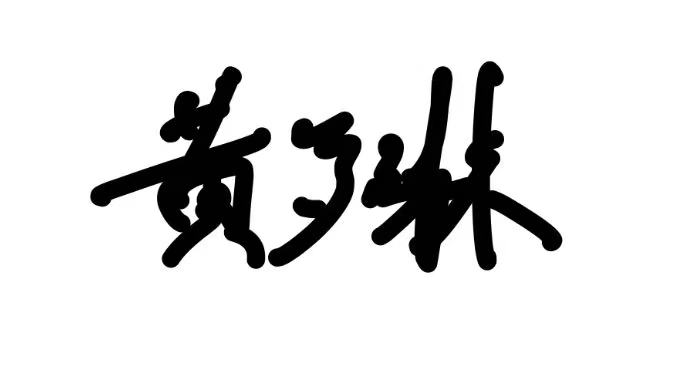
\includegraphics[width=1cm]{签字.jpg} & 评分: &\\
			\hline
			实验时间:& 2024/9/20 & 教师签名:&\\
			\hline
		\end{tabularx}
	\end{table}
	% ---
	
	% 小标题
	\section{ D2 材料真空兼容性测试和等离子特性研究\quad\heiti 实验记录}
	\subsection{真空的获取}
	\subsubsection{实验内容}
启动机械泵观察记录真空度(真空计压强) 随时间(5 分钟) 的变化。 机械泵先
		抽真空压强低于 10 Pa 后, 启动分子泵观察记录真空度( 真空计压强) 随时间的变
		化, 待分子泵达到额定转速(约需 8 分钟) 后再观察记录(5 分钟) 。停止分子泵观察记录真空度(真空计压强) 随时间的变化(分子泵转速降为零约需 8 分钟) 。 待分子泵完全停止后, 关闭机械泵, 记录真空度(真空计压强) 随时
		间的变化(5 分钟) 。

	\subsubsection{实验数据}
	

	\begin{longtable}{|c|c|c|c|c|c|c|c|}
		\caption{实验数据表} \\
		
		\hline
		\textbf{时间(S)} & \textbf{气压大小} & \textbf{时间(S)} & \textbf{气压大小} & \textbf{时间(S)} & \textbf{气压大小} & \textbf{时间(S)} & \textbf{气压大小} \\
		\hline
		\endfirsthead
		
		\hline
		\textbf{时间(S)} & \textbf{气压大小} & \textbf{时间(S)} & \textbf{气压大小} & \textbf{时间(S)} & \textbf{气压大小} & \textbf{时间(S)} & \textbf{气压大小} \\
		\hline
		\endhead
		
		\hline
		\multicolumn{8}{r}{续表} \\
		\endfoot
		
		\hline
		\endlastfoot
		
		26 & 8.10E+01 & 36 & 2.00E+01 & 46 & 1.40E+01 & 56 & 1.10E+01 \\ 
		\hline
		66 & 9.80E+00 & 76 & 8.80E+00 & 85 & 7.80E+00 & 100 & 6.90E+00 \\ 
		\hline
		120 & 6.00E+00 & 140 & 5.30E+00 & 160 & 4.80E+00 & 180 & 4.40E+00 \\ 
		\hline
		200 & 4.00E+00 & 220 & 3.70E+00 & 240 & 3.50E+00 & 260 & 3.30E+00 \\ 
		\hline
		280 & 3.10E+00 & 300 & 2.90E+00 & 320 & 2.80E+00 & 340 & 2.60E+00 \\ 
		\hline
		360 & 2.50E+00 & 380 & 2.40E+00 & 400 & 7.20E-01 & 420 & 2.00E-01 \\ 
		\hline
		440 & 6.90E-02 & 460 & 3.80E-02 & 480 & 3.30E-02 & 500 & 2.60E-02 \\ 
		\hline
		520 & 2.10E-02 & 540 & 1.60E-02 & 560 & 1.20E-02 & 580 & 9.80E-03 \\ 
		\hline
		600 & 8.20E-03 & 620 & 6.90E-03 & 640 & 6.10E-03 & 660 & 4.90E-03 \\ 
		\hline
		680 & 4.70E-03 & 700 & 4.40E-03 & 720 & 4.40E-03 & 740 & 4.20E-03 \\ 
		\hline
		760 & 4.10E-03 & 780 & 3.90E-03 & 800 & 3.80E-03 & 820 & 3.70E-03 \\ 
		\hline
		840 & 3.50E-03 & 860 & 3.40E-03 & 880 & 3.30E-03 & 900 & 3.20E-03 \\ 
		\hline
		920 & 3.10E-03 & 940 & 3.10E-03 & 960 & 3.00E-03 & 980 & 2.90E-03 \\ 
		\hline
		1000 & 2.80E-03 & 1020 & 2.70E-03 & 1040 & 2.60E-03 & 1060 & 2.60E-03 \\ 
		\hline
		1080 & 2.50E-03 & 1100 & 2.30E-03 & 1120 & 2.30E-03 & 1140 & 2.20E-03 \\ 
		\hline
		1160 & 2.20E-03 & 1180 & 2.20E-03 & 1200 & 2.20E-03 & 1220 & 2.20E-03 \\ 
		\hline
		1240 & 2.20E-03 & 1260 & 2.10E-03 & 1280 & 2.10E-03 & 1300 & 2.10E-03 \\ 
		\hline
		1320 & 2.10E-03 & 1340 & 2.20E-03 & 1360 & 2.20E-03 & 1380 & 2.30E-03 \\ 
		\hline
		1400 & 2.40E-03 & 1420 & 2.50E-03 & 1440 & 2.80E-03 & 1460 & 3.20E-03 \\ 
		\hline
		1480 & 3.70E-03 & 1500 & 4.60E-03 & 1520 & 7.00E-03 & 1540 & 1.90E-02 \\ 
		\hline
		1560 & 3.20E-02 & 1580 & 4.10E-02 & 1600 & 5.00E-02 & 1620 & 1.00E-01 \\ 
		\hline
		1640 & 1.70E-01 & 1660 & 2.40E+00 & 1680 & 2.60E+00 & 1700 & 2.80E+00 \\ 
		\hline
		1720 & 3.10E+00 & 1740 & 3.30E+00 & 1760 & 3.50E+00 & 1780 & 3.70E+00 \\ 
		\hline
		1800 & 3.80E+00 & 1820 & 4.00E+00 & 1840 & 4.20E+00 & 1860 & 4.40E+00 \\ 
		\hline
		1880 & 4.60E+00 & 1900 & 4.80E+00 & 1920 & 5.00E+00 & 1940 & 5.20E+00 \\ 
		\hline
	
		\end{longtable}
		
		
		
\subsection{真空帕邢实验}
\subsubsection{实验内容}
\begin{itemize}
    \item 测量两电极之间的实际间距。
    \item 检查放电管与电源之间的电路连接是否可靠;电压调节旋扭是否处于最小位置;气体流量调节旋扭是否处于最小位置。
    \item 检查高压电源开关,分子泵电源开关是否处于断开状态。
    \item 打开电源总开关。
    \item 开启机械泵,抽真空至 2-3Pa,过程大约需要 10 分钟。
    \item 调节减压阀,使得流量计前气压在 0-1 大气压之间(指导教师准备)。
    \item 调节流量计的通气流量,使放电管内气压达到 20Pa。
    \item 观察真空计数据并记录。
    \item 打开高压电源开关。
    \item 调节电源的电压输出,快速增至 200V,然后缓慢升高电压,直至气体发生击穿现象。读取击穿时的电压,记录气压和电压的数值。随后将电压降至 0V,为下一次测量做好准备。在减小电压过程中,观察放电熄灭电压,并注意其与击穿电压的差别。
    \item 注意事项:
        \begin{itemize}
            \item 增加电压的过程中,密切观察放电管电压表头和击穿电压表头的示数。
            \item 每个气压下,至少要重复 3 次测量,以三次击穿电压测量值之间的偏差不大于 15\% 为成功测量,确保数据可靠。
            \item 在气压较高时,击穿前后放电管的电压会明显下降。接近击穿时的放电管电压为气体击穿电压。
        \end{itemize}
    \item 增加气体流量,使气压升高至 30Pa,重复之前的测量步骤。
    \item 依次增加气体流量,每次增加 10Pa 左右,重复测量,直到气压达到 100Pa。记录 8 组实验数据。
    \item 减少气压,回复至 20Pa,重复测量。
    \item 依次减小气压,每次减少 2Pa,记录数据,直至气压达到 4Pa。测量并记录 7-8 组数据。
    \item 实验完毕后,调节气体流量控制旋钮至最小位置,调节电压至最小值,依次关闭电压、机械泵和电源开关。
\end{itemize}
\subsubsection{实验数据}\begin{table}[H]
	\centering
	\caption{气压与击穿电压实验数据}
	\begin{tabular}{rrrrr}
		\toprule
		气压/Pa & 击穿电压1/V & 击穿电压2/V & 击穿电压3/V & 击穿电压平均值/V \\
		\midrule
			4 &     864 &     843 &     875 &       860 \\
			6 &     650 &     642 &     656 &       649 \\
			8 &     554 &     532 &     532 &       539 \\
		   10 &     500 &     498 &     476 &       491 \\
		   12 &     474 &     472 &     478 &       475 \\
		   14 &     459 &     450 &     437 &       449 \\
		   16 &     475 &     467 &     456 &       466 \\
		   18 &     476 &     474 &     456 &       469 \\
		   20 &     474 &     477 &     481 &       477 \\
		   30 &     540 &     536 &     529 &       535 \\
		   40 &     580 &     573 &     567 &       573 \\
		   50 &     636 &     627 &     637 &       633 \\
		   60 &     669 &     660 &     676 &       668 \\
		   70 &     706 &     711 &     711 &       709 \\
		   80 &     741 &     743 &     738 &       741 \\
		   90 &     774 &     772 &     775 &       774 \\
		  100 &     795 &     796 &     801 &       797 \\
		\bottomrule
	\end{tabular}
	\end{table}
	
	
\subsection{等离子光谱}
观察气体放电(发光) 现象, 利用光纤光谱仪研究气体放电产生的等离子体光谱特
性, 获得等离子体基本参数, 了解等离子体物理的基本知识。
\subsubsection{实验数据}
\begin{table}[htbp]
    \centering    
	\caption{等离子体光谱实验数据}
    \begin{tabular}{|c|c|c|c|}
        \hline
        \textbf{气压 (Pa)} & \textbf{气体} & \textbf{电压 (V)} & \textbf{电流 (uA)} \\ \hline
        12  & 空气  & 446  & 600  \\ \hline
        24  & 氦气  & 725  & 600  \\ \hline
        24  & 氖气  & 437  & 600  \\ \hline
        24  & 氩气  & 328  & 600 \\ \hline
    \end{tabular}

\end{table}
\subsection{四极质谱实验}
\subsubsection{实验步骤}
\begin{itemize}
    \item 因该试验台为综合性试验台,实验前需检查真空腔体与电源之间的电路连接是否可靠;电压调节旋扭置于最小位置,气体流量置于合适状态。
    
    \item 检查高压电源开关以及分子泵是否处于断开状态,检查四极质谱仪电源是否连接,数据线是否连接电脑。
    
    \item 当机械泵抽取压强至 10Pa 以下后,才能打开分子泵电源。等待 5 秒钟后,按下分子泵电源面板上的绿色按钮,进行分子泵运行(此时转速会从 450 转降至 68 转左右进行自检,后开始从 68 转上升至 450 转)。
    
    \item 观察真空计显示屏,待分子泵抽取至 5.0E-2Pa 以下再打开四极质谱仪。
    
    \item 继续抽取真空,待压强低于 $10^{-3}$Pa 后,可通过气阀加入适量 He、Ne、Ar 等气体,便于通过软件观察各质谱图。(切记加入后压强勿超过 5.0E-2Pa,若超过该压强,则需继续抽气至低于该值后才能通过软件打开质谱仪灯丝,否则将严重损坏质谱仪灯丝)。
    
    \item 打开测试软件 VAccuRay3.0 进行实验。
\end{itemize}
\subsubsection{实验数据}
\begin{table}[H]
    \centering
    \begin{tabular}{|c|c|}
        \hline
        \textbf{气体} & \textbf{气压 (Pa)} \\ \hline
        无(本底谱) & $7.8 \times 10^{-4}$ \\ \hline
        空气        & $2.5 \times 10^{-2}$ \\ \hline
        氦气        & $3.0 \times 10^{-3}$ \\ \hline
        氖气        & $1.6 \times 10^{-2}$ \\ \hline
        氩气        & $3.2 \times 10^{-2}$ \\ \hline
    \end{tabular}
    \caption{不同气体的气压数据}
\end{table}
	\subsection{实验过程遇到问题及解决办法}
	\begin{enumerate}
		\item 实验中有些实验数据存在较大误差,通过增加实验次数,得到多组正确的实验数据后再进行下一步实验。
		\item 在四极质谱实验中,实验仪器出现了问题,在经过老师的帮助后,完成了实验仪器的测量和数据的导出。
	\end{enumerate}
	
	% 分析与讨论	
	\clearpage
	
	% 顶栏
	\begin{table}
		\renewcommand\arraystretch{1.7}
		\begin{tabularx}{\textwidth}{|X|X|X|X|}
			\hline
			专业:& 物理学 &年级:& 2022级\\
			\hline
			姓名: &黄罗琳  & 学号:&22344001 \\
			\hline
			日期:& 2024/9/27 & 评分: & \\
			\hline
		\end{tabularx}
	\end{table}
	% ---
	
	% 小标题
	\section{ D2 材料真空兼容性测试和等离子特性研究\quad\heiti 分析与讨论}
	
	\subsection{实验数据分析}
	\subsubsection{真空的获取}
	根据实验所得到压强随时间的变化数据,绘制出如下曲线
	\begin{figure}[{H}]
		\centering
		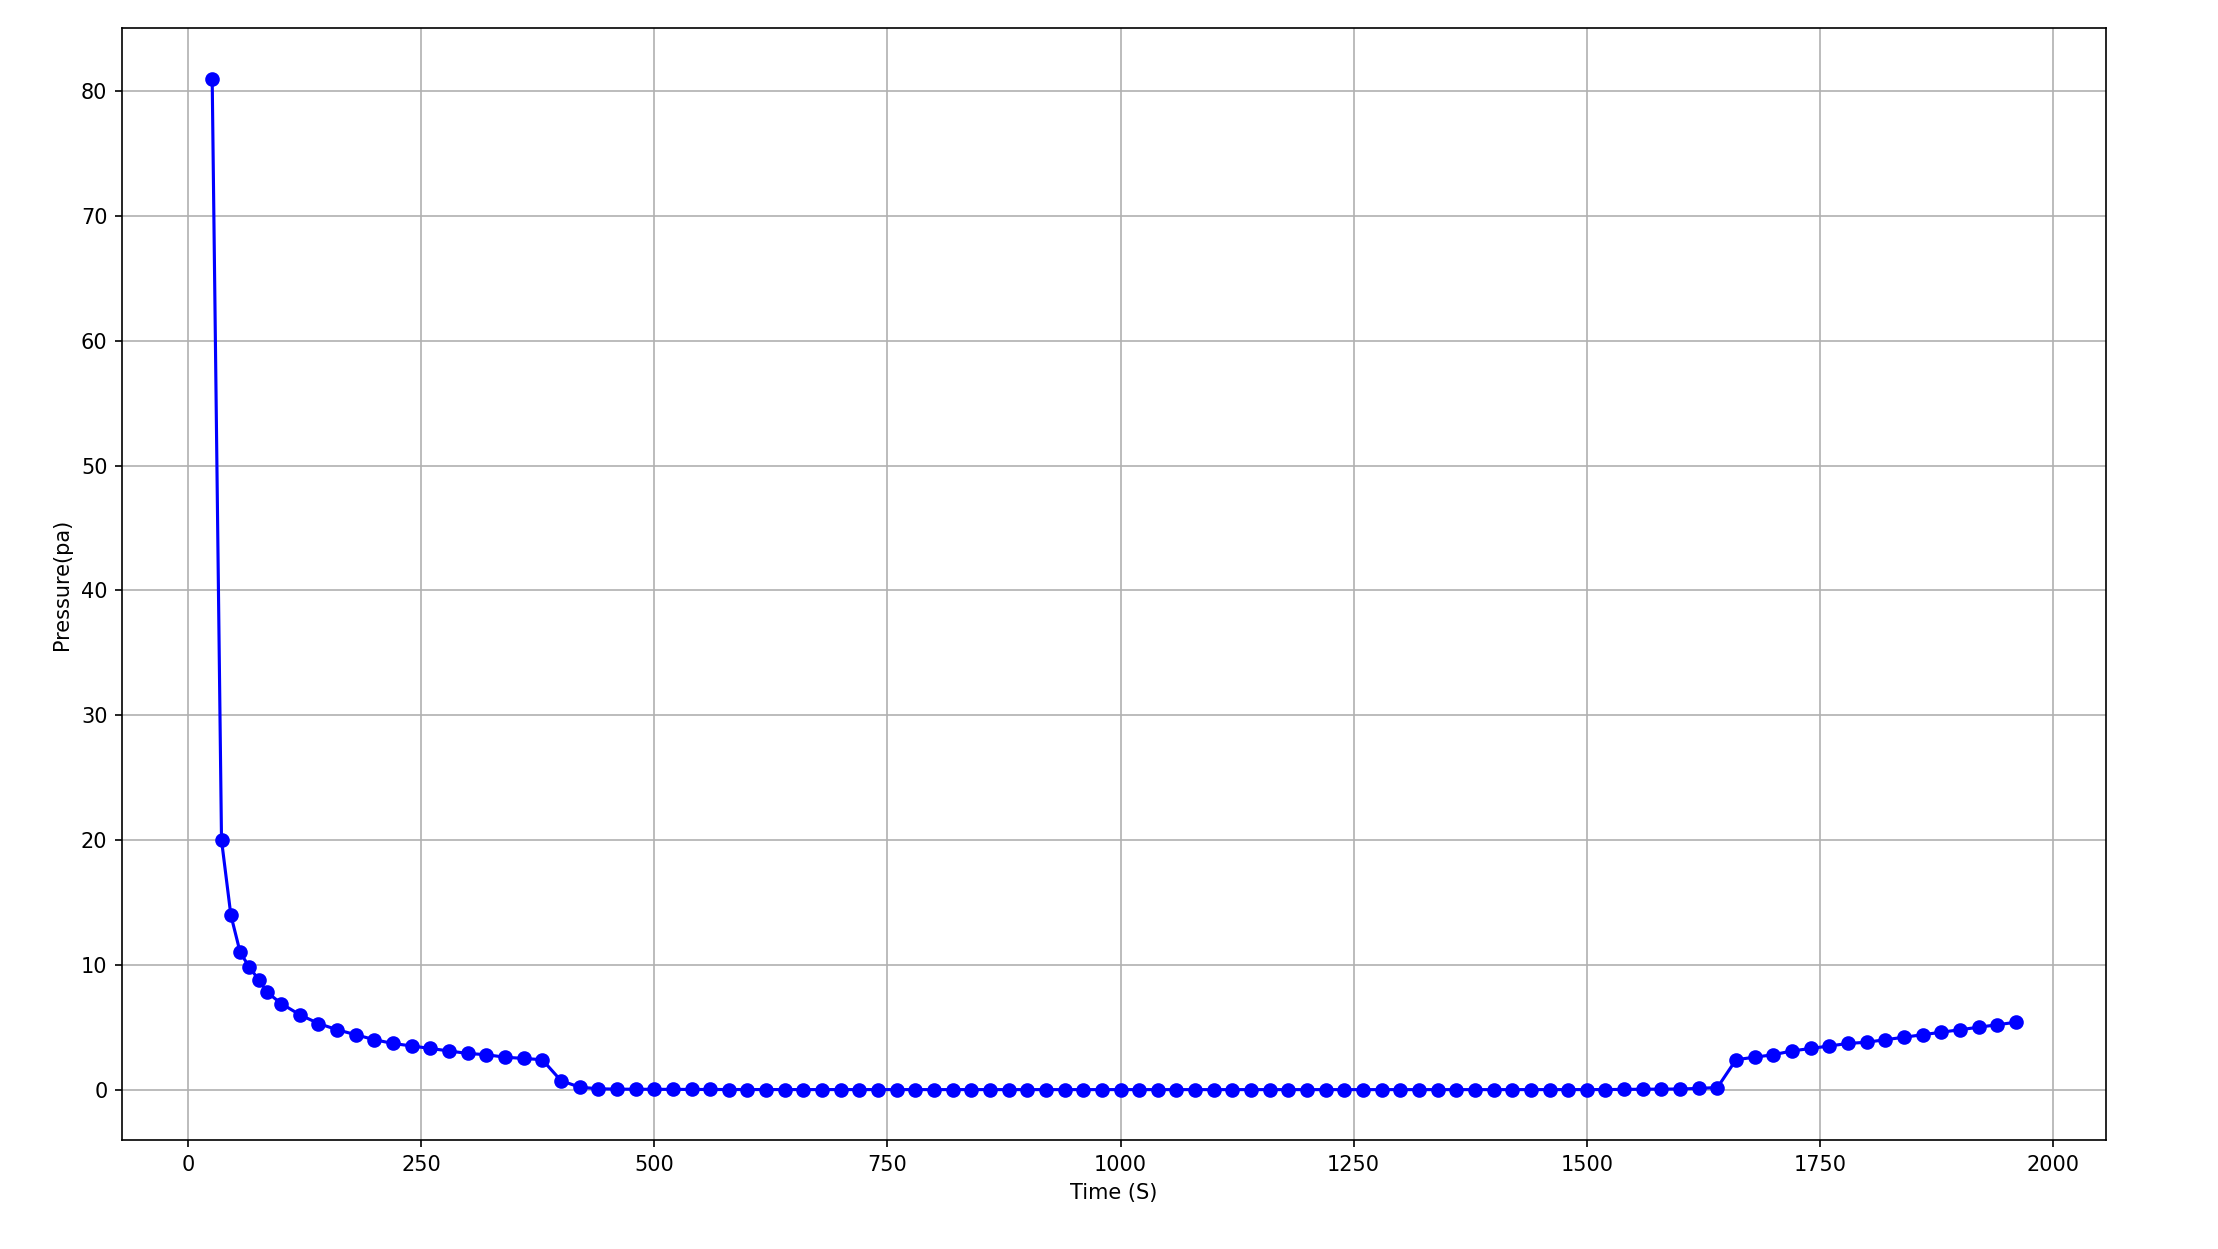
\includegraphics[width=0.6\linewidth]{pt.png}
		\caption{压强随时间变化曲线}
		\label{}
	\end{figure}


	实验开始时,我们首先开启机械泵,系统内的气压开始迅速下降。由于机械泵的抽气效率较高,在初始阶段气压迅速降低,在短时间内从大气压下降到接近10Pa。然而,当气压降到10Pa左右时,气体分子密度逐渐减少,机械泵的抽气速度随之变慢。随着抽气的持续进行,压强逐步下降至大约1.8Pa左右,此时压强难以再显著降低,系统达到了机械泵的极限真空状态。

为了进一步降低系统内的气压,我们开启了分子泵。分子泵启动后,气压再次迅速下降,由于其对低压条件下的抽气效率较高,系统内的气压快速降低。随着分子泵的转速逐渐达到额定值,气压的下降速度逐渐放缓。最终气压降到了2.6E-3Pa,这时系统已经进入了高真空状态,达到实验所需的真空水平。

随后,我们关闭了分子泵,系统内的气压开始缓慢上升。这是因为在关闭分子泵后,仍有微量气体分子进入真空腔体,同时分子泵停止运行后其内的残余气体释放出来,导致气压有所回升。随着分子泵的转速逐步下降,气压在其完全停止工作时上升到了5.4Pa。

接下来,我们关闭了机械泵,但是由于实验记录视频的缺失,导致此部分的实验记录数据缺失,但是此处的图像曲线应与实验最开始打开机械泵的曲线相同,即如图所示的压强随时间变化曲线应该是对称的。
	\subsubsection{真空帕邢实验}
	测量击穿电压与电极间隙和气压之间的关系,绘制帕邢曲线如下图所示。

\begin{figure}[{H}]
	\centering
	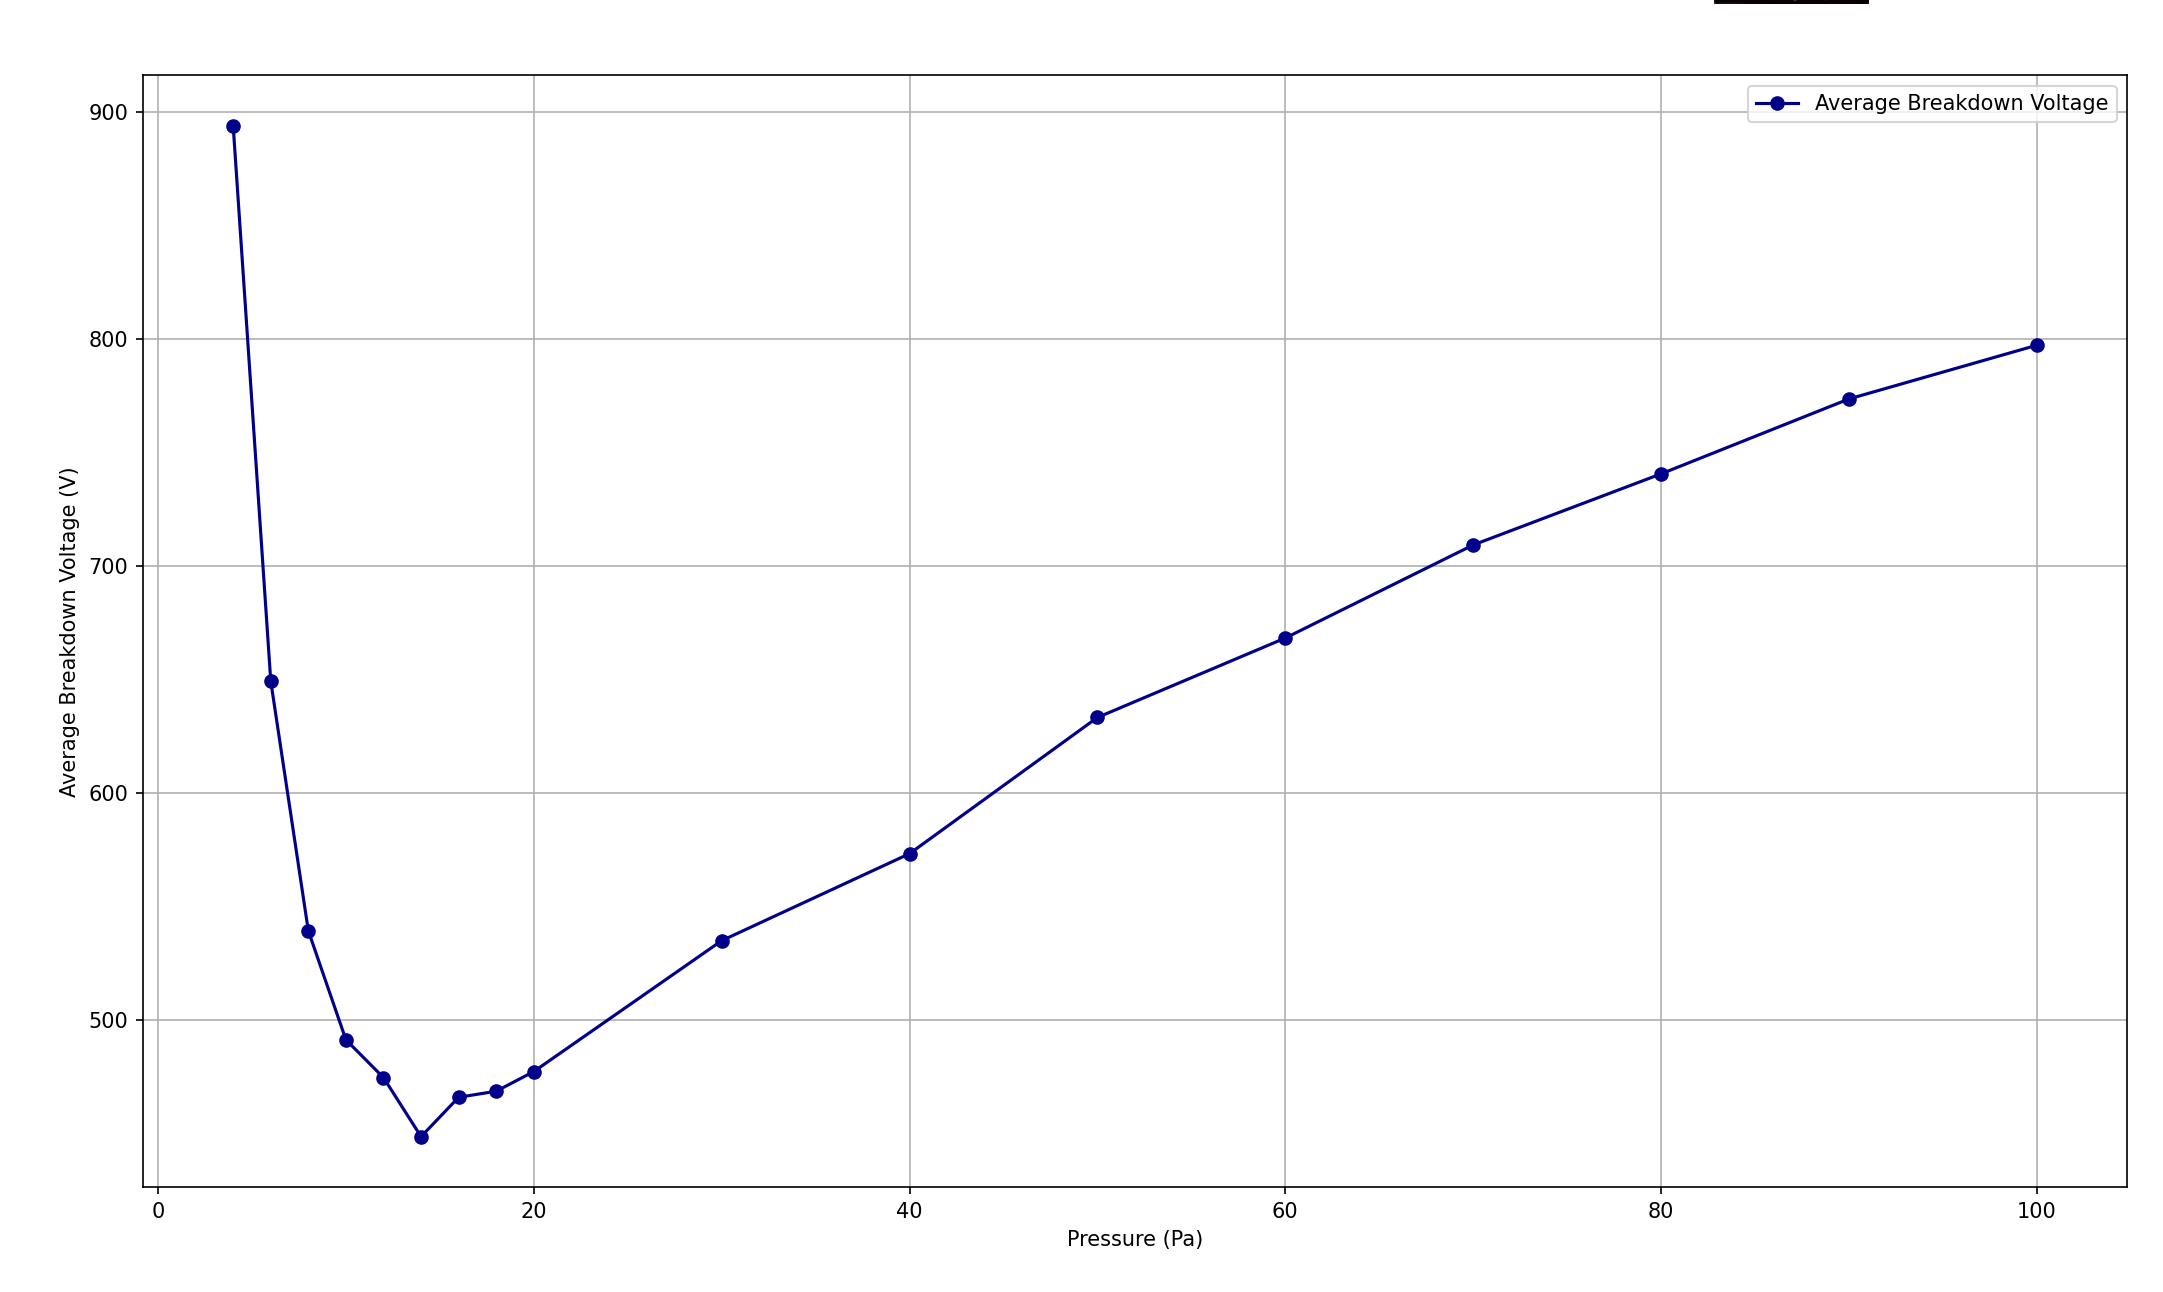
\includegraphics[width=0.5\linewidth]{px.png}
	\caption{帕邢曲线}
	\label{}
\end{figure}

	由图可见,曲线在特定的 $P$值时,有最小的击穿电压,满足帕邢定律。最小击穿电压为 449.0V,在电极间距 $48mm$ 的情况下最佳击穿条件为 $14Pa$ 的气压, 乘积为 $672Pa · mm$。
	
	\subsubsection{等离子体光谱}
	根据实验数据,绘制图像,并进行寻峰,最终找到峰对应的波长数据。
	\begin{figure}[{H}]
		\centering
		\begin{minipage}{0.45\linewidth}
			\centering
			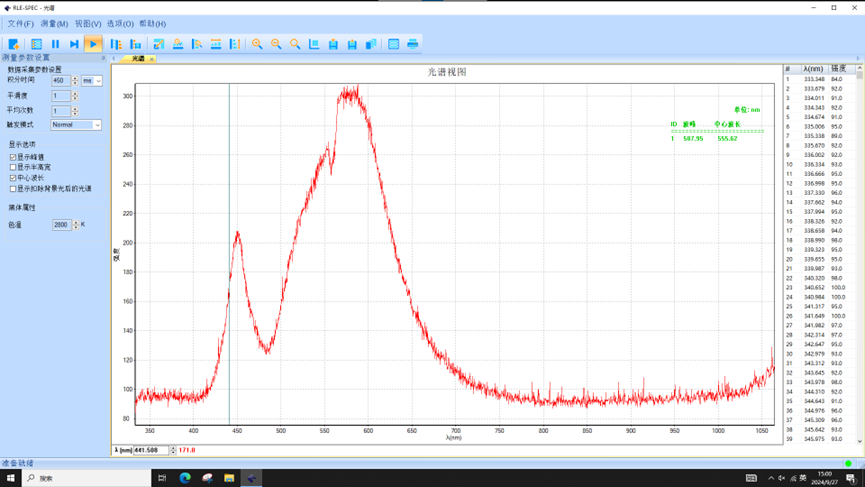
\includegraphics[width=\linewidth]{an.png}
			\caption{暗光谱}
		\end{minipage}
		\hspace{0.05\linewidth}
		\begin{minipage}{0.45\linewidth}
			\centering
			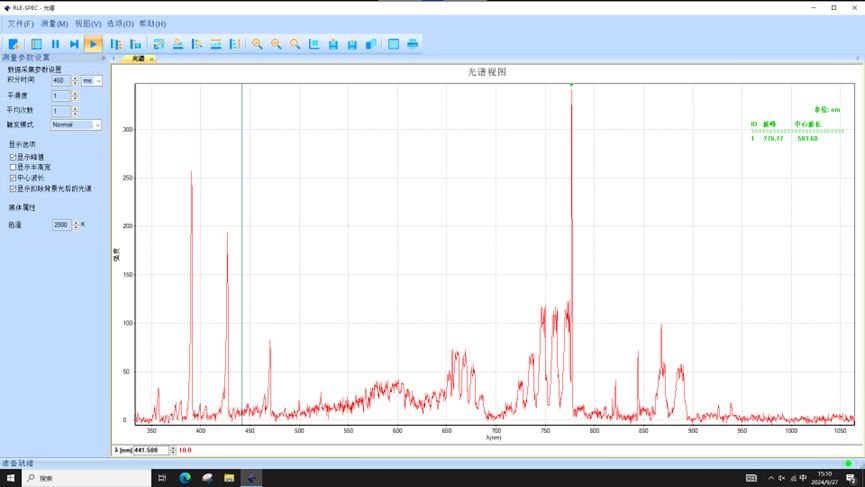
\includegraphics[width=\linewidth]{kongqi.png}
			\caption{空气 12pa 446v 600$\mu A$}
		\end{minipage}
	\end{figure}
	
	\begin{figure}[{H}]
		\centering
		\begin{minipage}{0.45\linewidth}
			\centering
			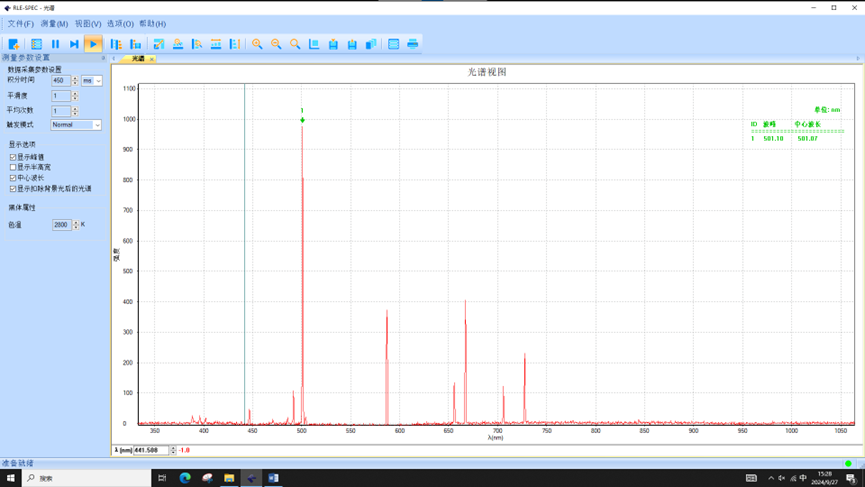
\includegraphics[width=\linewidth]{he1.png}
			\caption{氦气 24pa 725v 600$\mu A$}
		\end{minipage}
		\hspace{0.05\linewidth}
		\begin{minipage}{0.45\linewidth}
			\centering
			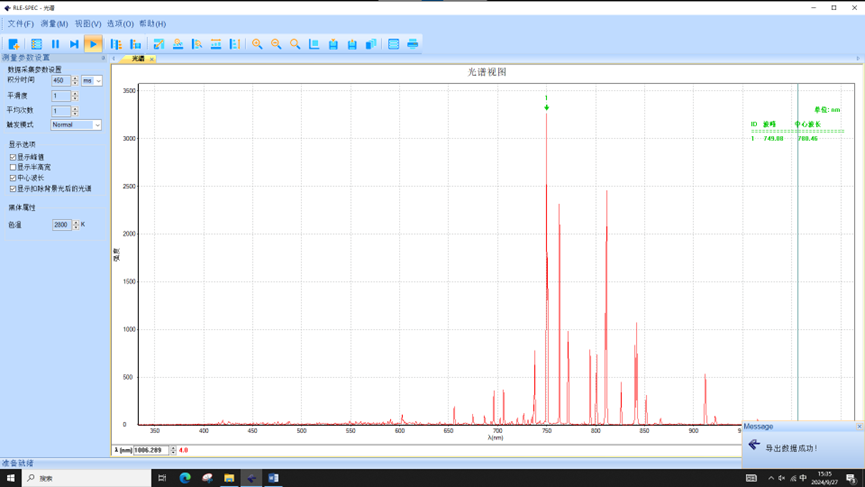
\includegraphics[width=\linewidth]{ar1.png}
			\caption{氩气 24pa 328v 600$\mu A$}
		\end{minipage}
	\end{figure}
	
	\begin{figure}[{H}]
		\centering
		\begin{minipage}{0.45\linewidth}
			\centering
			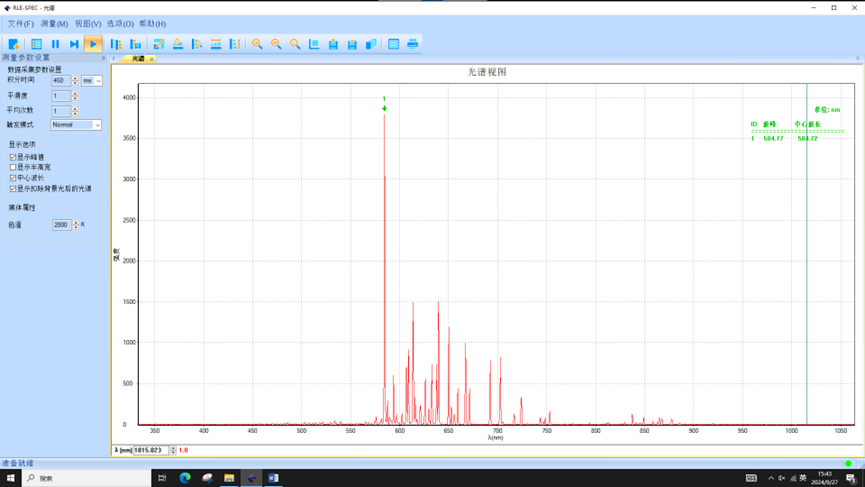
\includegraphics[width=\linewidth]{ne1.png}
			\caption{氖气 24pa 436v 600$\mu A$}
		\end{minipage}
		\hspace{0.05\linewidth}
		\begin{minipage}{0.45\linewidth}
			\centering
			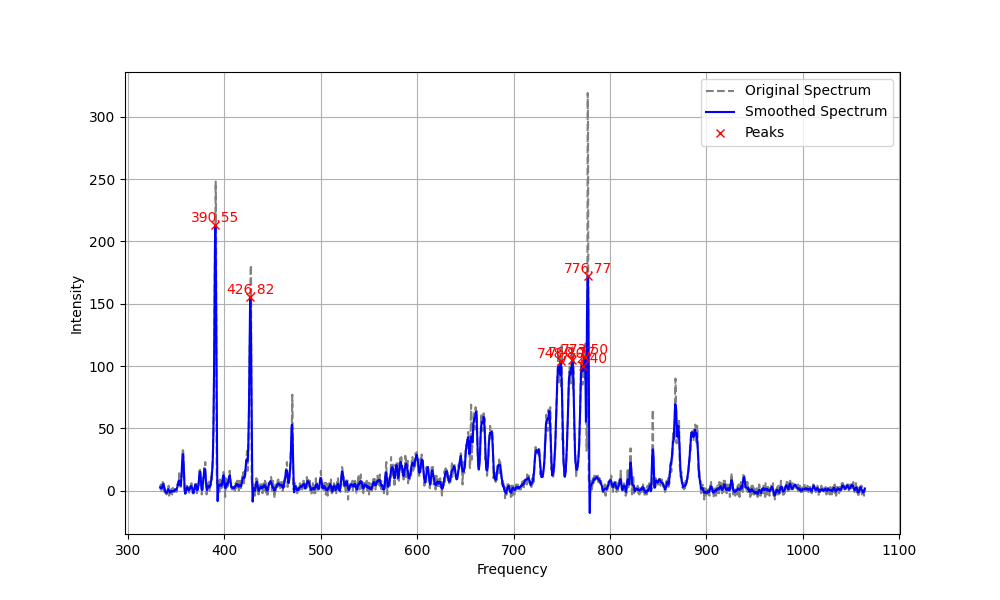
\includegraphics[width=\linewidth]{空气12pa446v600微安.txt_spectrum_filtered.png}
			\caption{空气光谱数据寻峰}
		\end{minipage}
	\end{figure}
	
	\begin{figure}[{H}]
		\centering
		\begin{minipage}{0.45\linewidth}
			\centering
			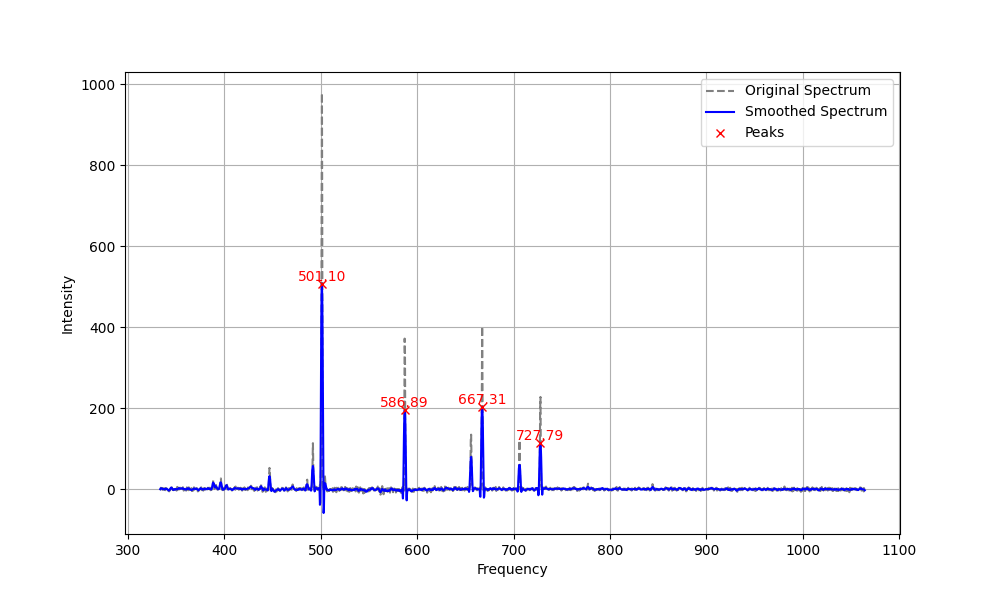
\includegraphics[width=\linewidth]{he 24pa 725v600微安.txt_spectrum_filtered.png}
			\caption{氦气光谱数据寻峰}
		\end{minipage}
		\hspace{0.05\linewidth}
		\begin{minipage}{0.45\linewidth}
			\centering
			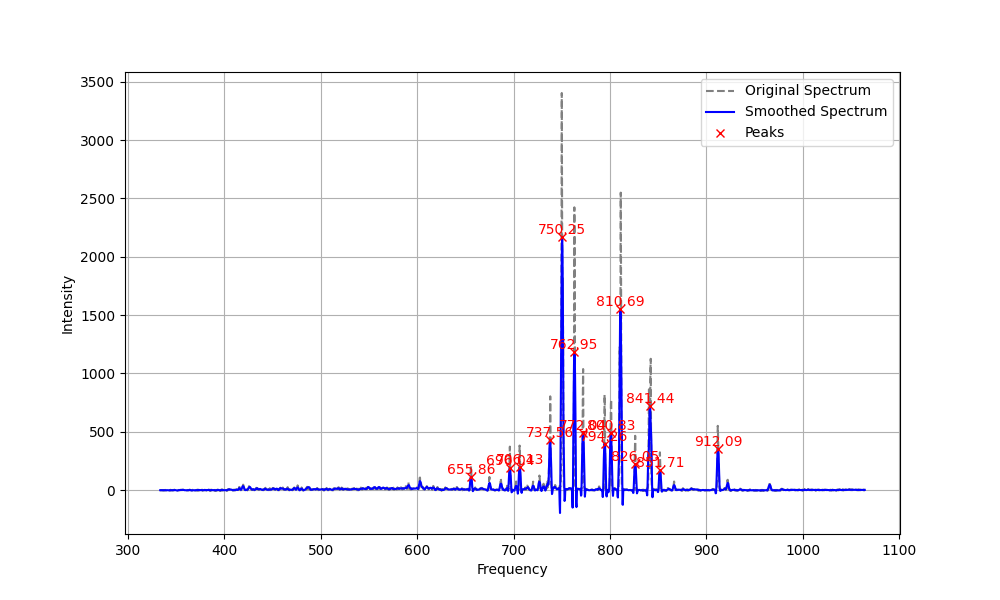
\includegraphics[width=\linewidth]{ar 24pa 328v600.txt_spectrum_filtered.png}
			\caption{氩气光谱数据寻峰}
		\end{minipage}
	\end{figure}
	
	\begin{figure}[{H}]
		\centering
		\begin{minipage}{0.45\linewidth}
			\centering
			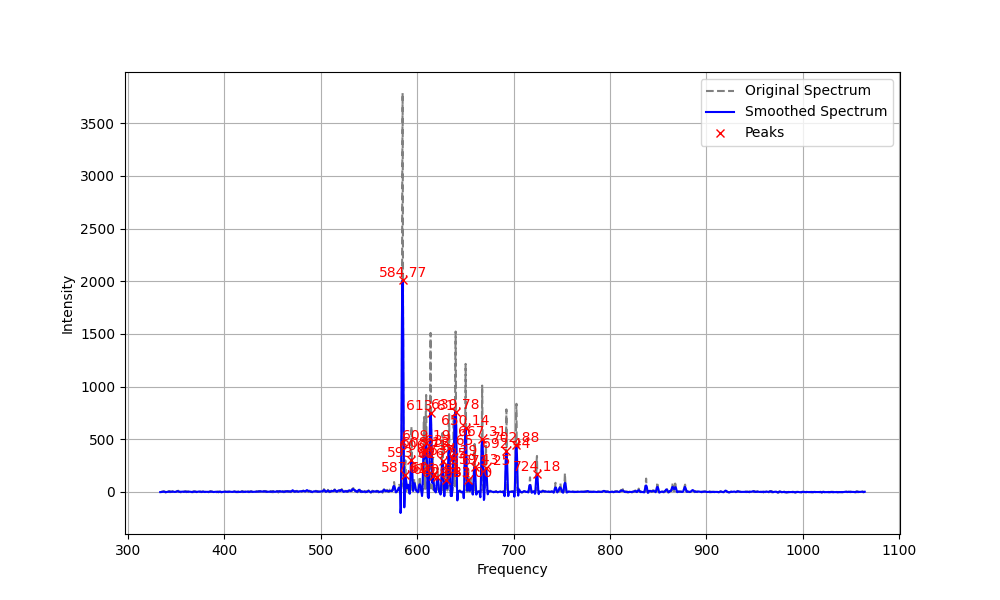
\includegraphics[width=\linewidth]{ne 24pa 437v600微安.txt_spectrum_filtered.png}
			\caption{氖气光谱数据寻峰}
		\end{minipage}
	\end{figure}
	
	\begin{itemize}
		\item 空气光谱:在实验中,空气帕邢放电发出紫色的光,这是由于空气分子在高压条件下被电离并激发所致。通过光谱分析,观察到强度较高的光谱峰值分别出现在 776.77 nm、390.55 nm 和 426.82 nm。776.77 nm 对应的是红外线,虽然它有较强的强度,但由于人眼对红外线不可见,因此实验中看不到这部分光。390.55 nm 和 426.82 nm 都属于紫外和蓝紫光谱段,两者的波长非常接近,产生了颜色类似的视觉效果,因此实验中看到的紫光是由这些光线共同作用所致。这个结果与实验观察到的现象相符,进一步验证了空气放电的发光机制。
		
		\item He 光谱:实验中,氦气帕邢放电发出较弱的绿光。光谱分析揭示了多个峰值,其中最强的几个峰分别出现在 501.10 nm、667.31 nm 和 586.89 nm。501.10 nm 对应的是绿光,并且在光谱中强度最高,这与实验中观察到的绿色光一致。667.31 nm 对应红光,虽然强度也比较高,但相对于绿光要弱一些,因此实验中红光并不显著。586.89 nm 是黄光的波长,虽然它也有一定强度,但它的光在实验中被绿光掩盖,显示不明显。这个光谱峰值的分布表明,氦气放电时发出的主要是绿光,符合实验观察的结果。
		
		\item Ne 光谱:在氖气帕邢放电实验中,观察到了红橙色的光。这与光谱分析的结果高度一致,强度较高的几个峰分别出现在 584.77 nm、639.78 nm 和 613.81 nm。584.77 nm 属于黄光范围,639.78 nm 对应的是红光,613.81 nm 属于橙光范围。由于这几种光线的强度接近,因此在实验中观察到的光呈现出红橙色的混合效果。这种颜色组合与氖灯发光时的典型现象一致,说明氖气在电场作用下的放电发光特性。
		
		\item Ar 光谱:实验中几乎观察不到氩气帕邢放电发出的可见光。通过光谱分析发现,氩气放电的主要峰值集中在近红外和红外波段。由于这些波段的光线在人眼可见光范围之外,因此实验中几乎看不到氩气的光发射。这与光谱数据完全符合,表明氩气在此实验条件下的电离发光集中于不可见的红外区域。
	\end{itemize}
	
	
	\subsubsection{四极质谱实验}

	
\begin{figure}[H]
	\centering
	% 第一组: Ar
	\begin{minipage}[H]{0.45\textwidth}
		\centering
		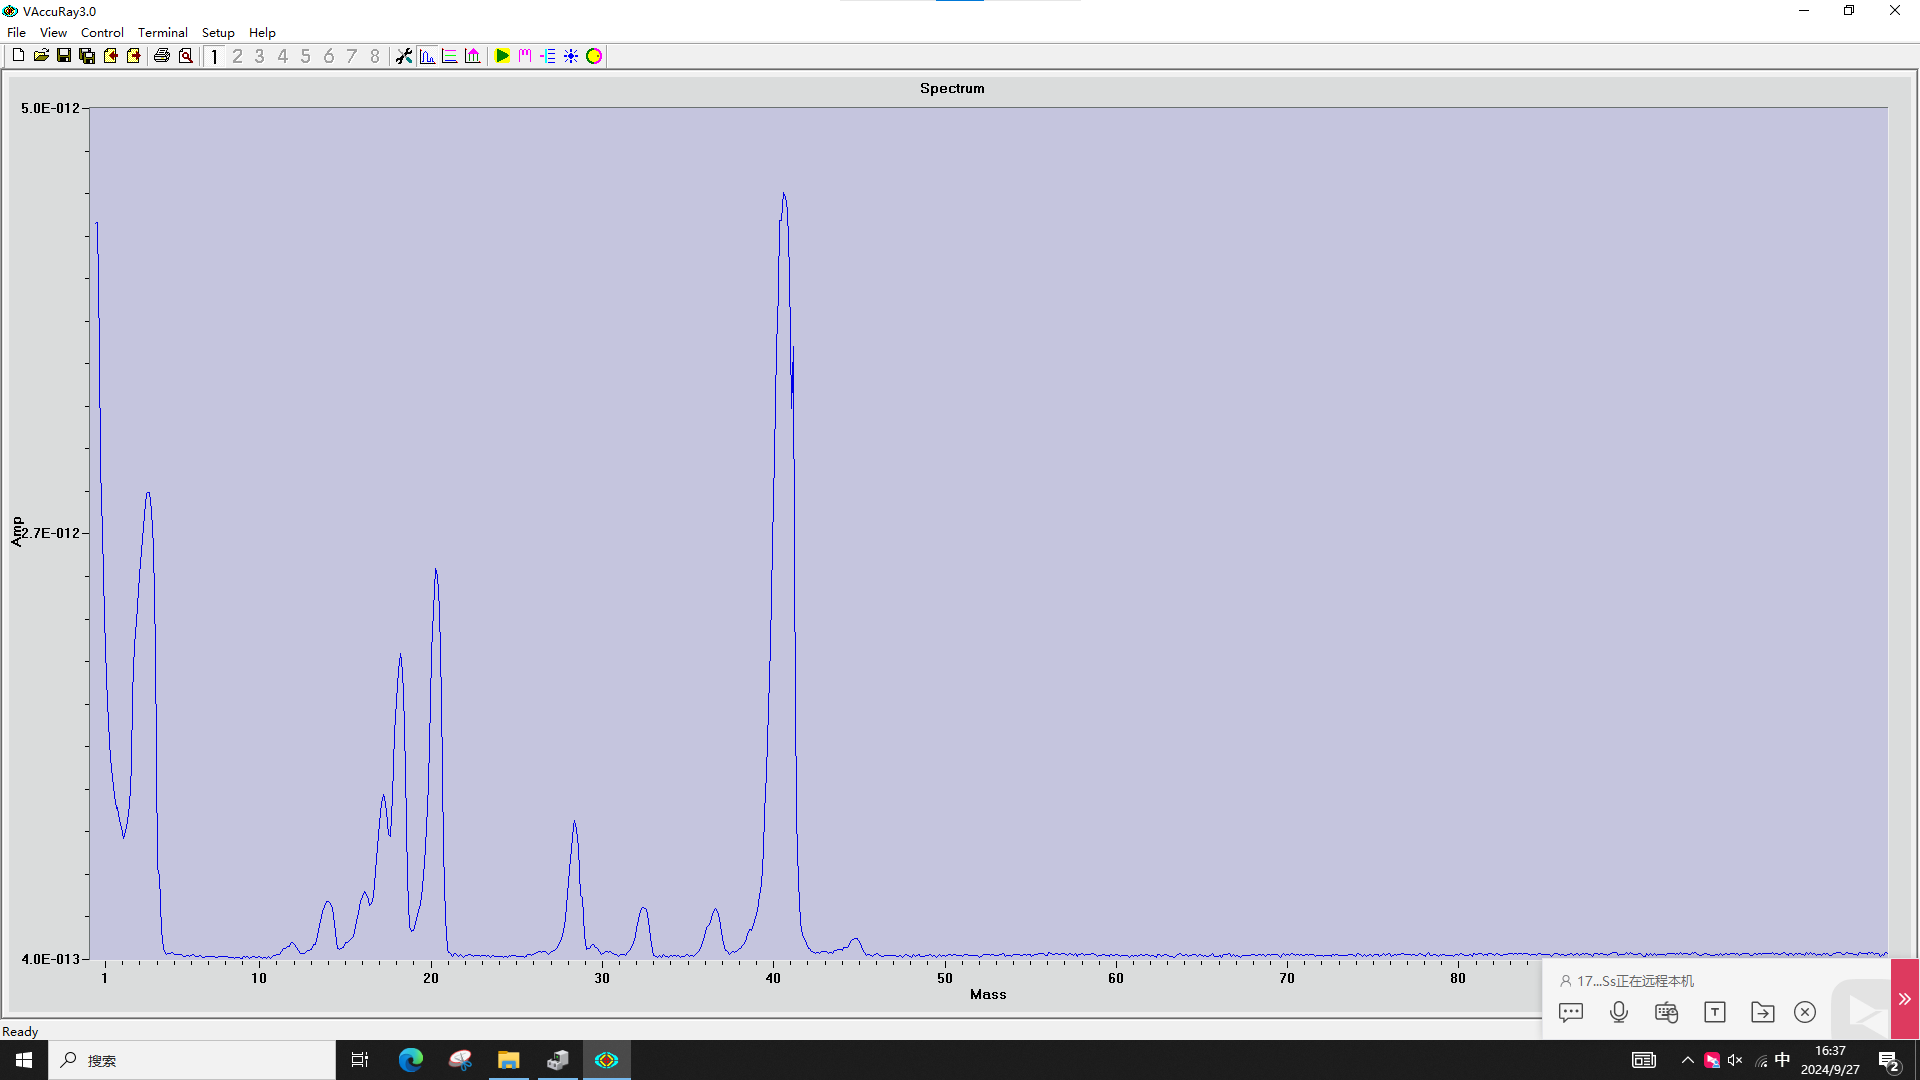
\includegraphics[width=\textwidth]{ar41.png}
		\caption{氩气质谱图}
	\end{minipage}
	\hfill
	\begin{minipage}[H]{0.45\textwidth}
		\centering
		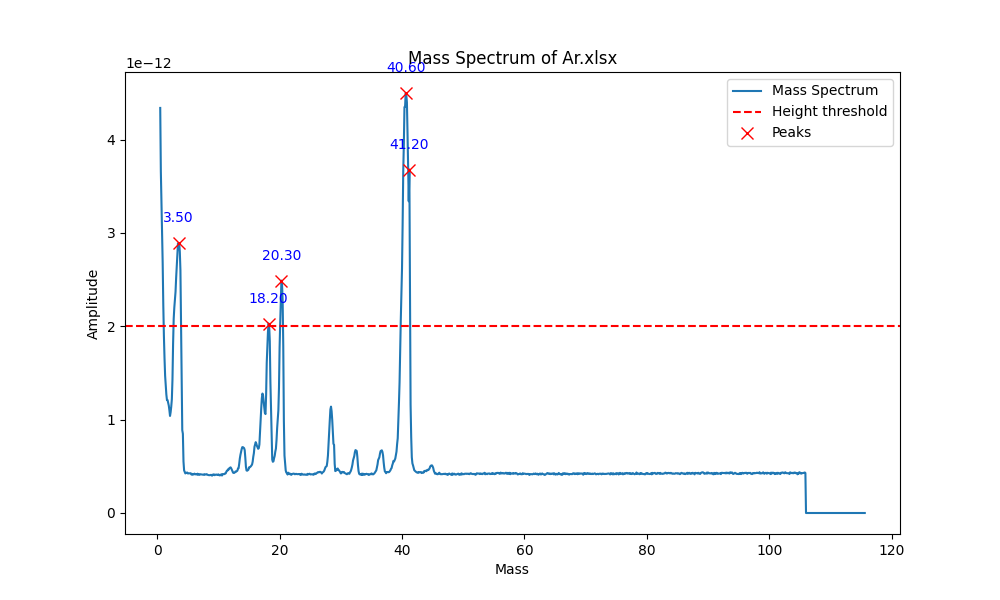
\includegraphics[width=\textwidth]{Ar42.png}
		\caption{氩气寻峰结果}
	\end{minipage}
\end{figure}

\begin{figure}[H]
	\ContinuedFloat
	% 第二组: He
	\begin{minipage}[H]{0.45\textwidth}
		\centering
		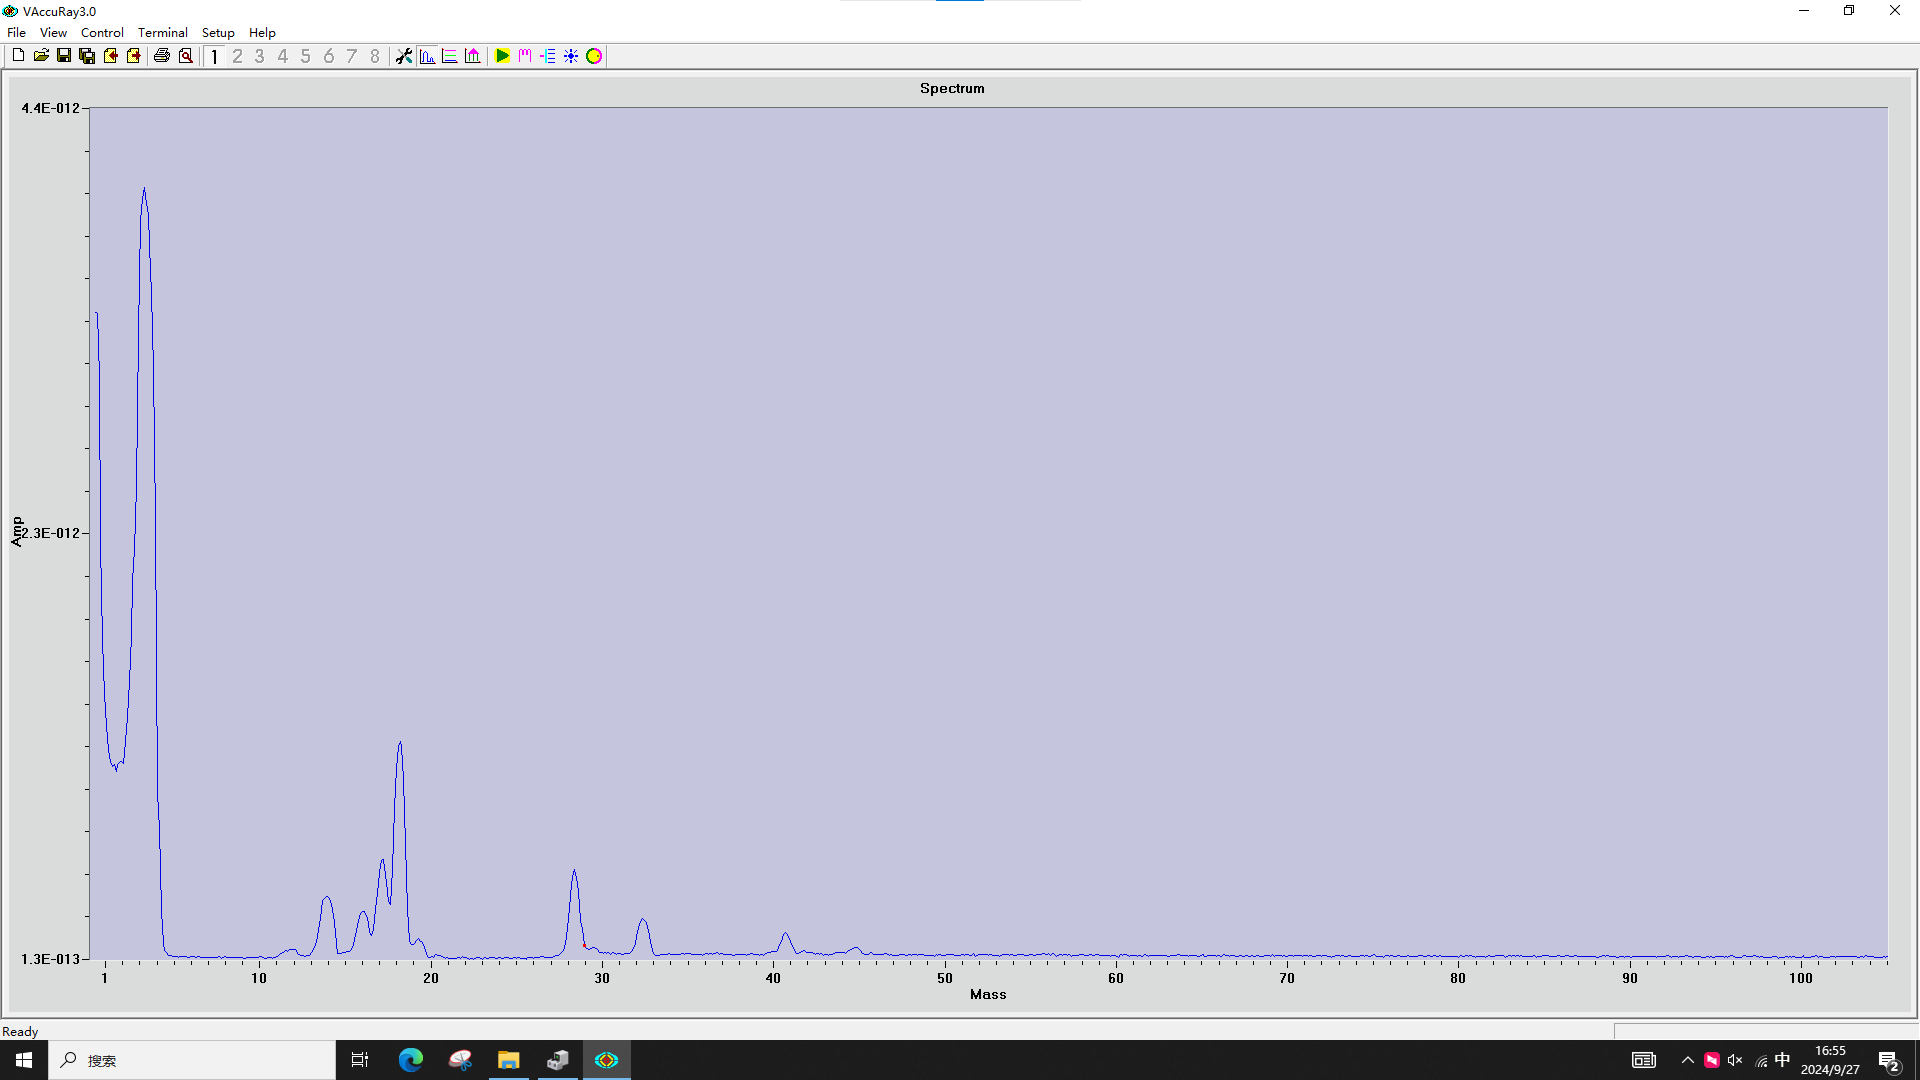
\includegraphics[width=\textwidth]{he41.png}
		\caption{氦气质谱图}
	\end{minipage}
	\hfill
	\begin{minipage}[H]{0.45\textwidth}
		\centering
		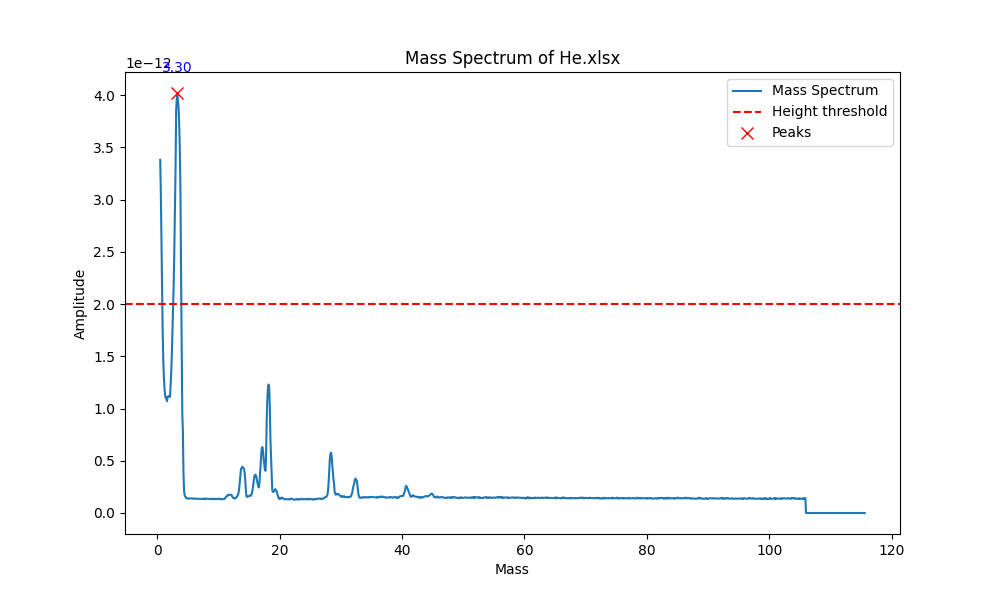
\includegraphics[width=\textwidth]{He42.png}
		\caption{氦气寻峰结果}
	\end{minipage}
\end{figure}

\begin{figure}[H]
	\ContinuedFloat
	% 第三组: Ne
	\begin{minipage}[H]{0.45\textwidth}
		\centering
		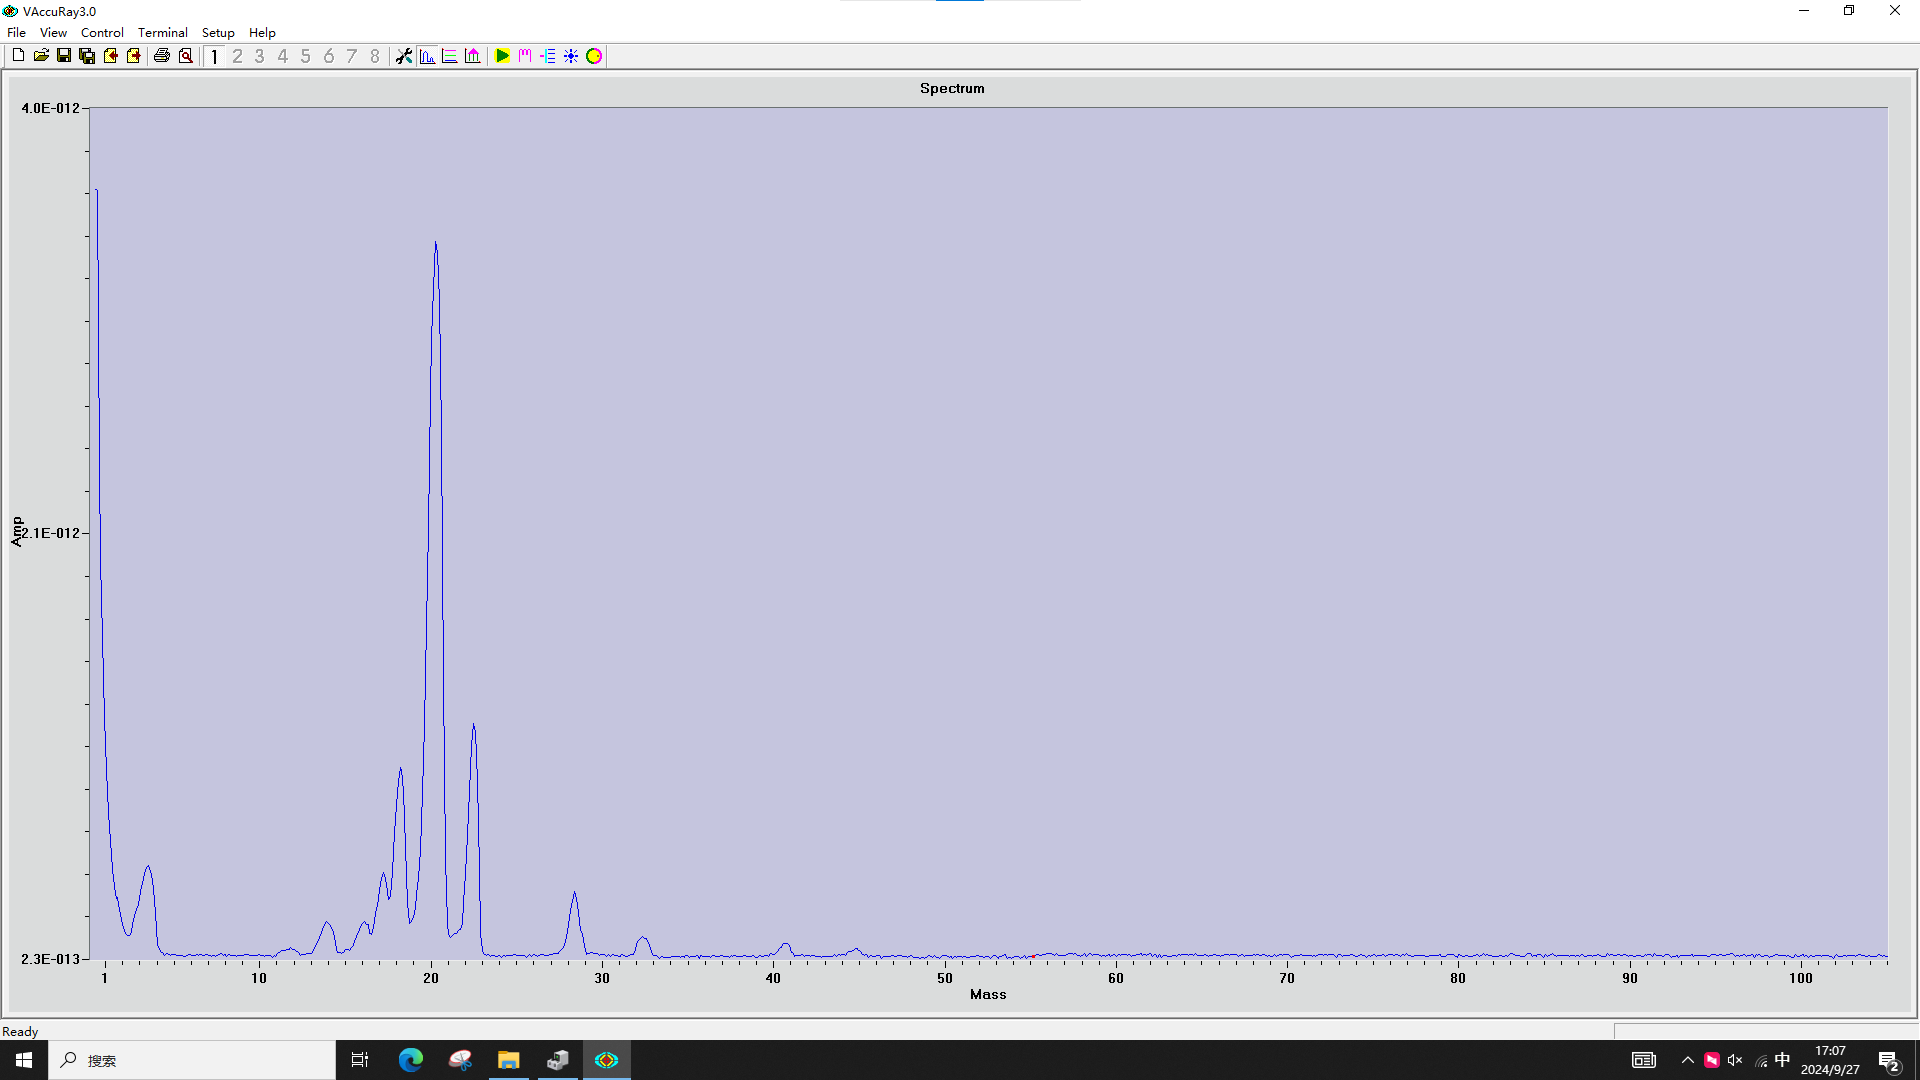
\includegraphics[width=\textwidth]{ne41.png}
		\caption{氖气质谱图}
	\end{minipage}
	\hfill
	\begin{minipage}[H]{0.45\textwidth}
		\centering
		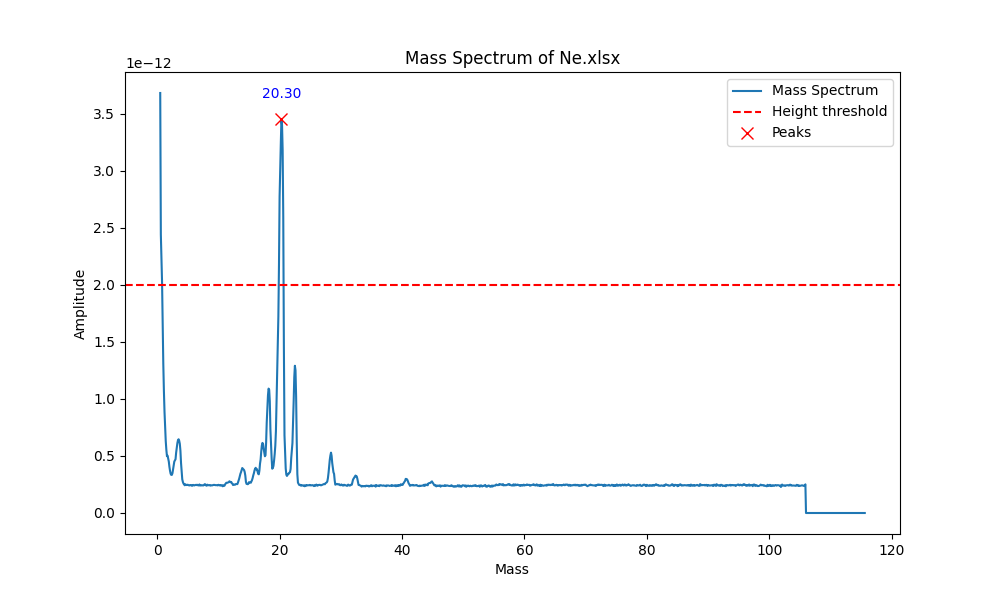
\includegraphics[width=\textwidth]{Ne42.png}
		\caption{氖气寻峰结果}
	\end{minipage}
\end{figure}

\begin{figure}[H]
	\ContinuedFloat
	% 第四组: 本底
	\begin{minipage}[H]{0.45\textwidth}
		\centering
		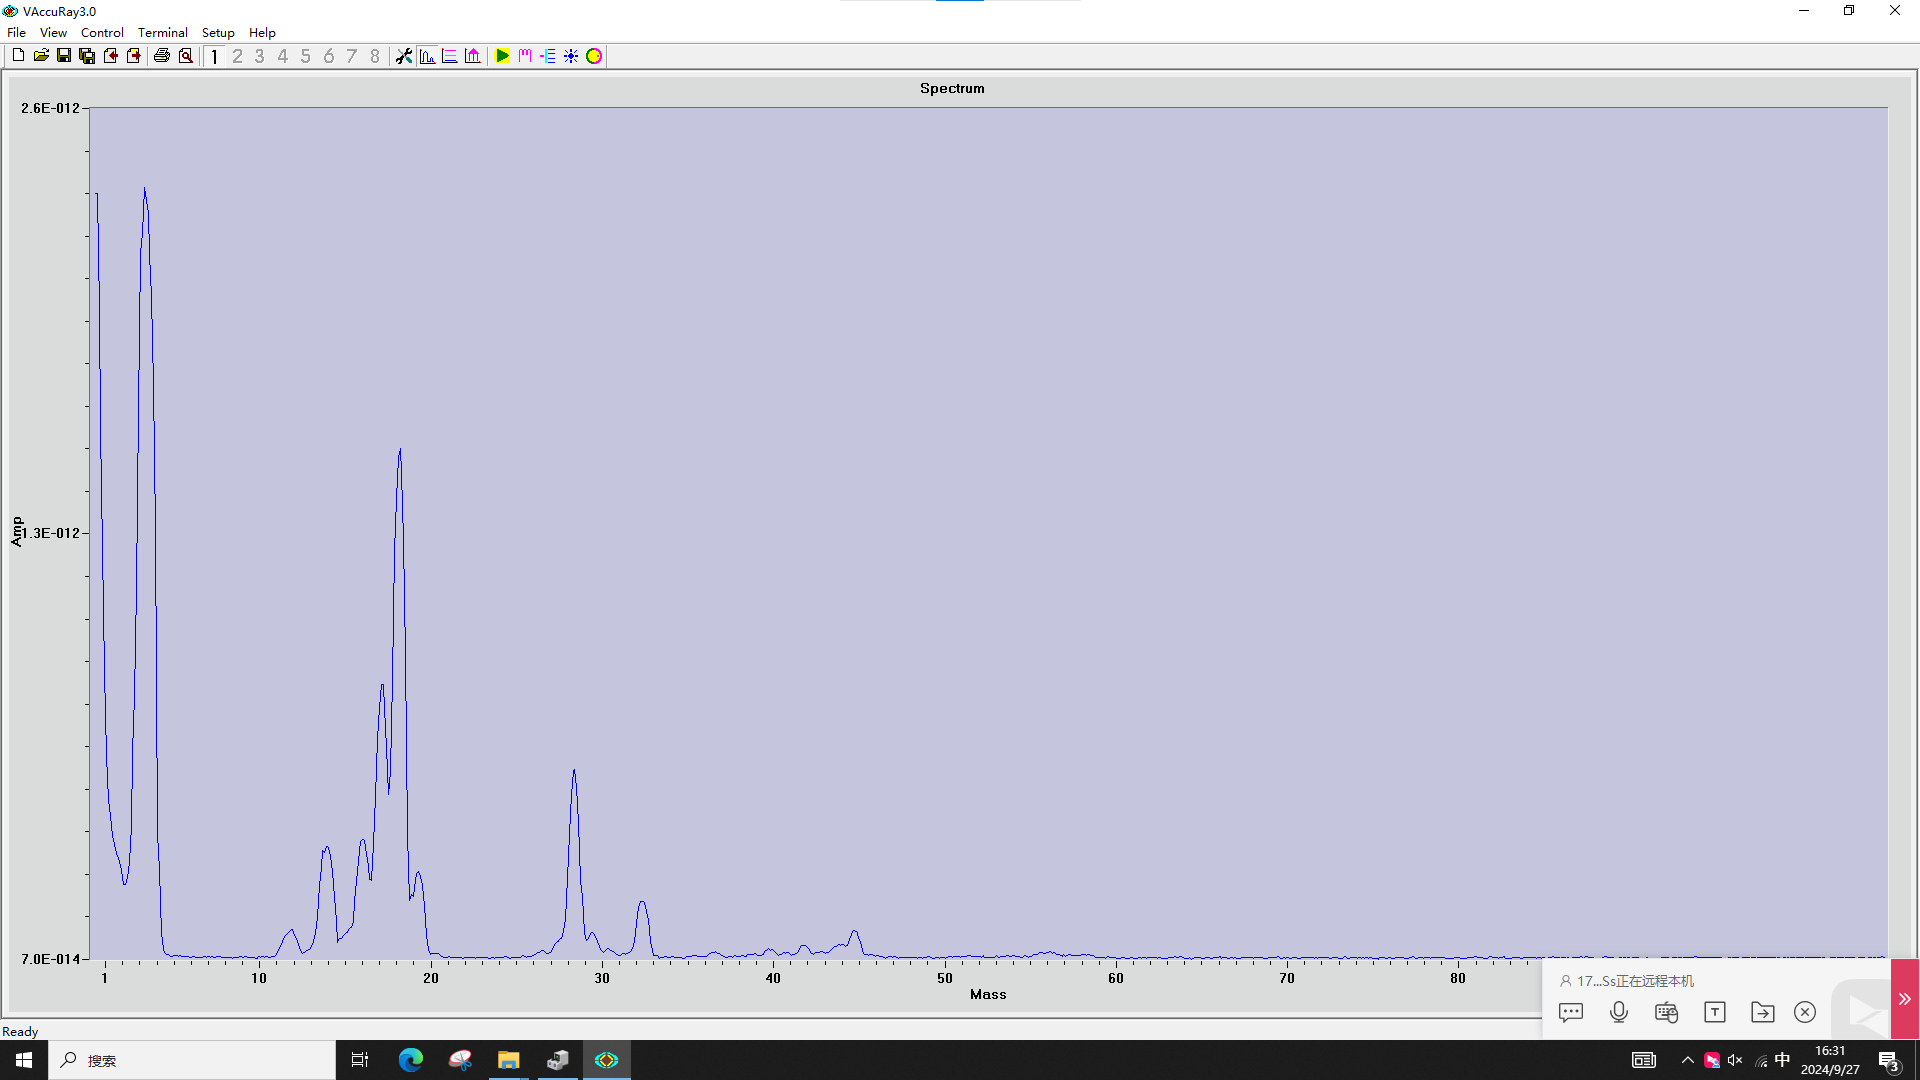
\includegraphics[width=\textwidth]{本底41.png}
		\caption{本底质谱图}
	\end{minipage}
	\hfill
	\begin{minipage}[H]{0.45\textwidth}
		\centering
		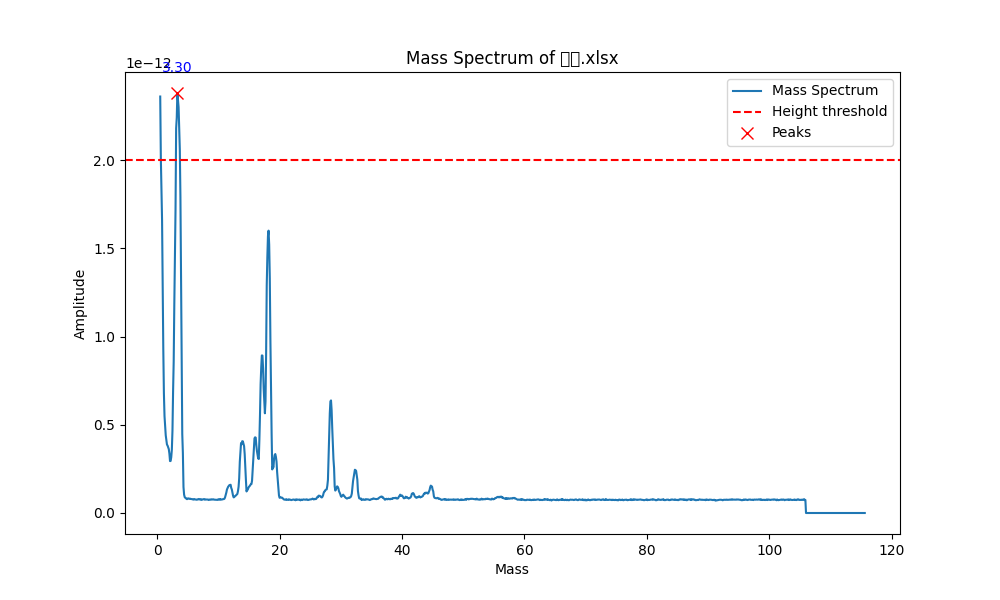
\includegraphics[width=\textwidth]{本底42.png}
		\caption{本底寻峰结果}
	\end{minipage}
\end{figure}

\begin{figure}[H]
	\ContinuedFloat
	% 第五组: 空气
	\begin{minipage}[H]{0.45\textwidth}
		\centering
		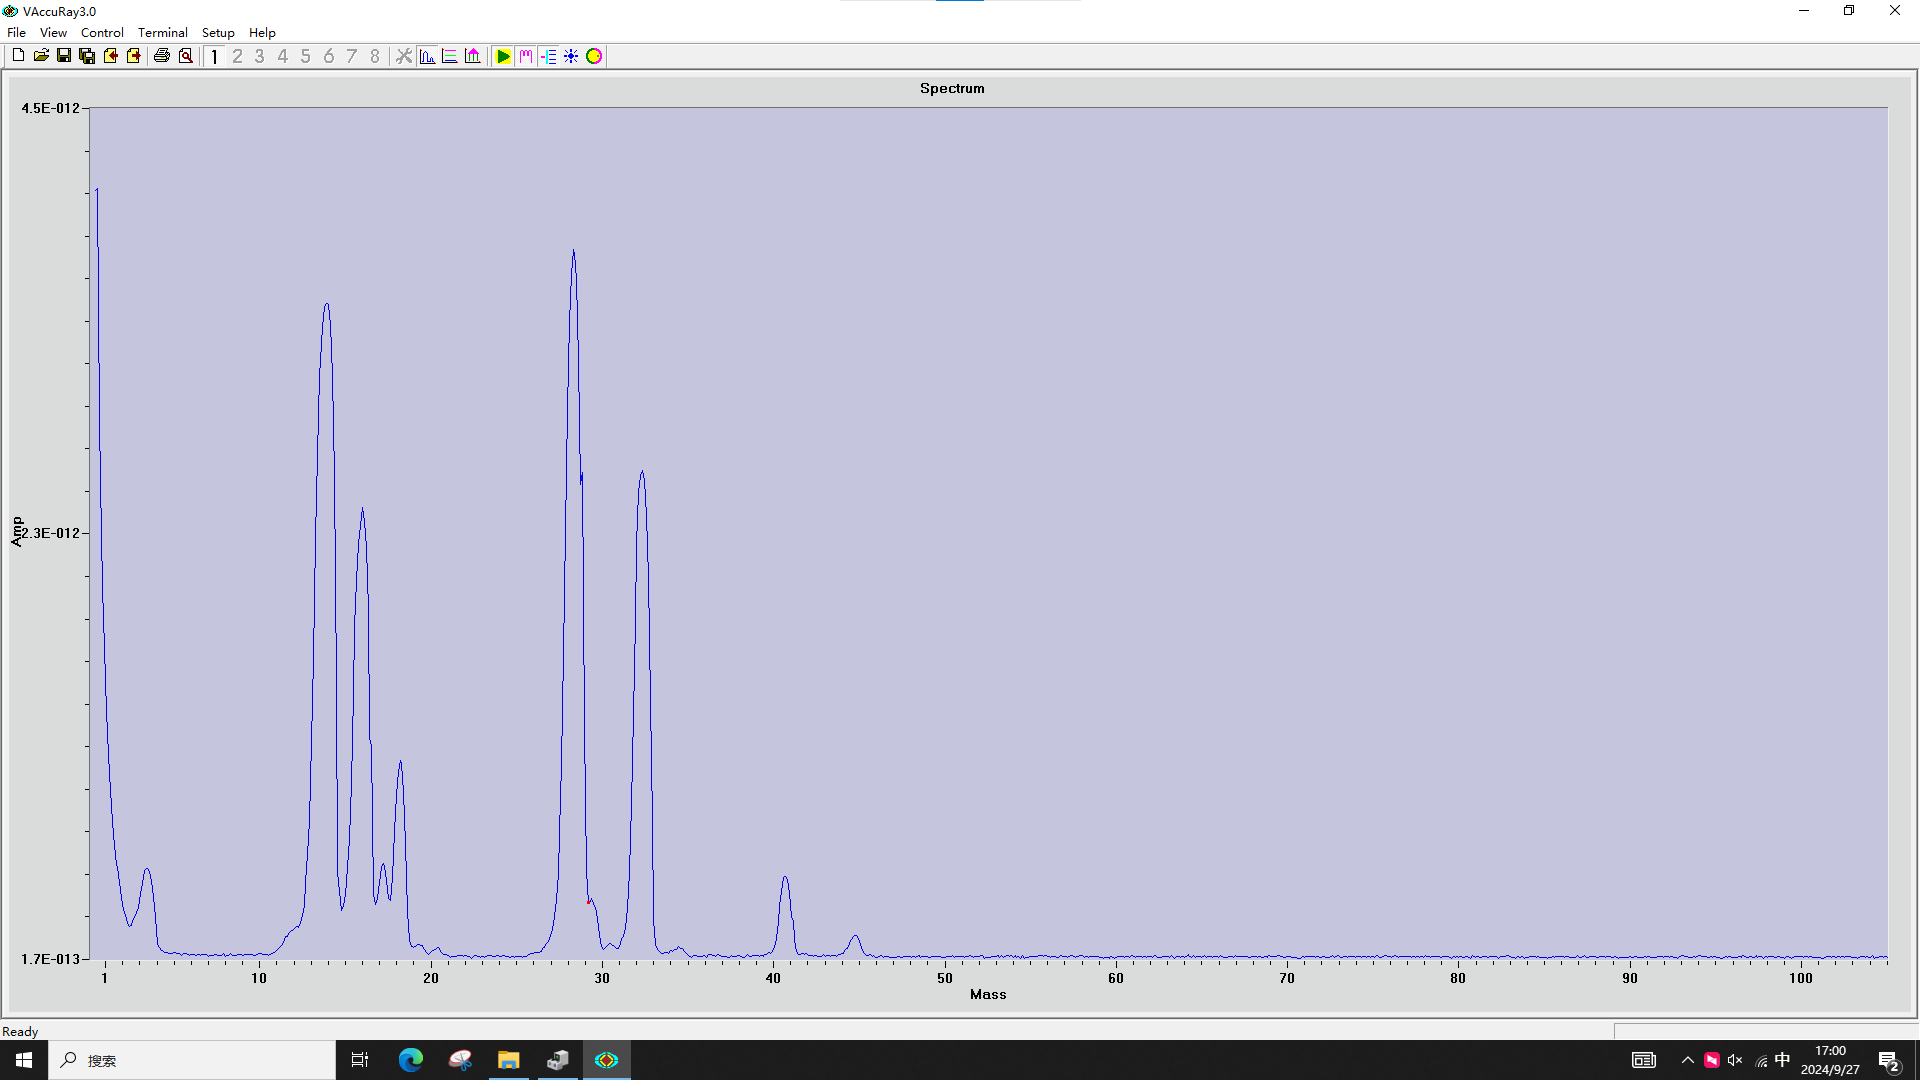
\includegraphics[width=\textwidth]{空气41.png}
		\caption{空气质谱图}
	\end{minipage}
	\hfill
	\begin{minipage}[H]{0.45\textwidth}
		\centering
		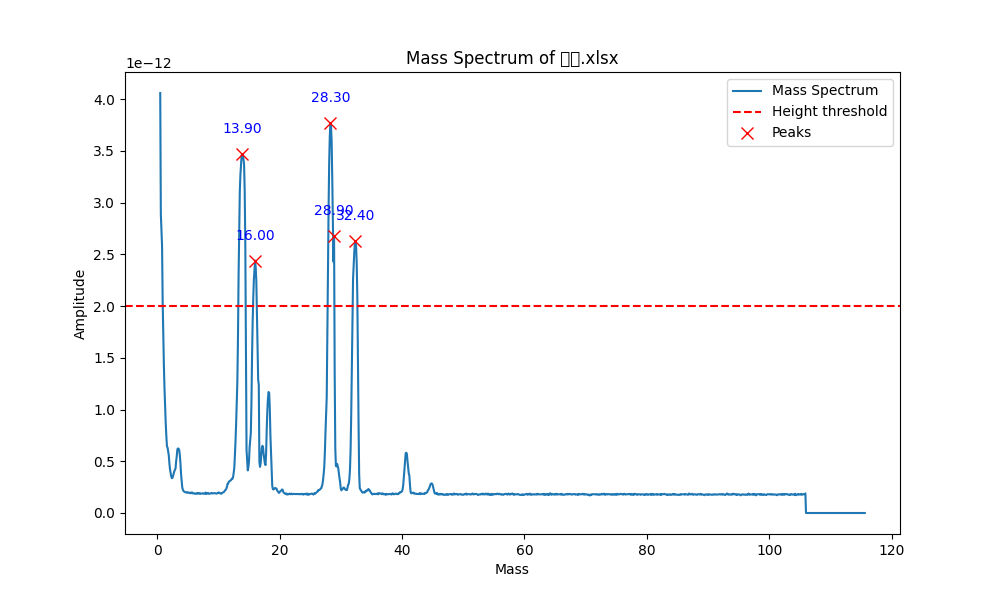
\includegraphics[width=\textwidth]{空气42.png}
		\caption{空气寻峰结果}
	\end{minipage}
\end{figure}






分析多个原理图可以得出如下结论:

\begin{itemize}
    \item \textbf{水的存在:} 
    
    在所有的质谱图中,均存在相对质量为 \textbf{$18.3$} 的峰。这与水的相对分子质量非常接近,推测该峰是由于设备内部残留的 \textbf{$H_2O$} 所导致的。后续分析中不再过多讨论此峰。

    \item \textbf{本底谱:}  
    
    本底质谱图中最高的峰对应相对质量为 \textbf{$18.3$},这与水的相对分子质量一致。因此,可以推测此时设备内部气体成分主要是 \textbf{水蒸气 ($H_2O$)}。

    \item \textbf{空气:}  ‘
    
    在空气的质谱图中,有三个主要峰:
    \begin{itemize}
        \item 相对质量 \textbf{$16.0$}:这可能与 \textbf{氧气 ($O_2$)} 分子的离解产物有关。
        \item 相对质量 \textbf{$28.3$}:与 \textbf{氮气 ($N_2$)} 的相对分子质量接近,是空气的主要成分之一。
        \item 相对质量 \textbf{$32.4$}:这与 \textbf{氧气 ($O_2$)} 的相对分子质量非常接近,因此可以确认空气的主要成分为 \textbf{氮气和氧气},以及少量的 \textbf{水蒸气 ($H_2O$)}。
    \end{itemize}

    \item \textbf{氦气:}  
    
    氦气质谱图中的最高峰对应的相对质量为 \textbf{$4.3$},这与氦的相对原子质量 \textbf{$4$} 非常接近。可以确认此时设备内部的气体成分主要为 \textbf{氦气 ($He$)}。

    \item \textbf{氖气:}  
    
    氖气质谱图中的最高峰对应相对质量为 \textbf{$20.3$},这与氖的相对原子质量非常接近,说明此时设备内的气体主要为 \textbf{氖气 ($Ne$)}。此外,还存在一个较小的峰,位于相对质量 \textbf{$18.3$} 处,说明设备中可能还残留了一定量的 \textbf{水蒸气 ($H_2O$)}。

    \item \textbf{氩气:}  
    
    氩气质谱图中的最高峰对应相对质量为 \textbf{$40.6$},这与氩的相对原子质量 \textbf{$40$} 非常接近,说明此时设备内的气体成分主要为 \textbf{氩气 ($Ar$)}。同样,另一个较小的峰位于 \textbf{$18.3$} 处,推测这也是由于设备内残留的 \textbf{水蒸气 ($H_2O$)} 所导致的。

\end{itemize}
Resolution 为 100 时,各气体波峰宽度明显增加,此时四极质谱的灵敏度相对增加,而精确度下降。
\begin{figure}[{H}]
	\centering
	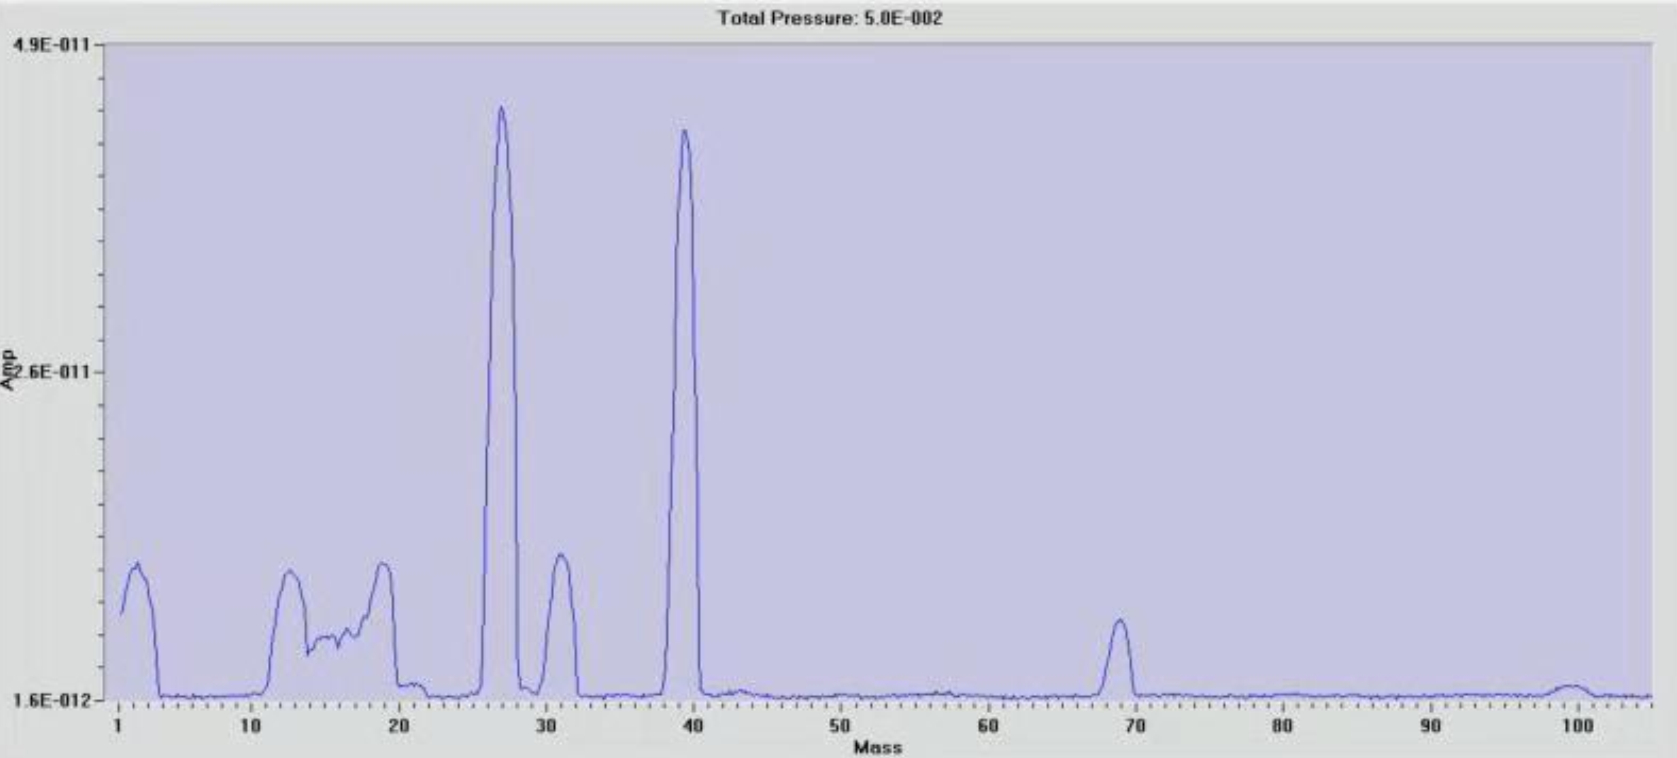
\includegraphics[width=0.4\linewidth]{1000.png}
	\caption{Resolution100}
	\label{}
\end{figure}
	% 实验后思考题
	\subsection{实验思考题}
	
	%思考题1
	\begin{question}
		真空度(真空计压强) 随时间变化反映了真空系统的什么特性?
	\end{question}
	\begin{itemize}
		\item \textbf{抽气效率与泵的性能}:
		\begin{itemize}
			\item 初始阶段,机械泵的高抽气效率使得系统内压迅速下降,这表明机械泵在大气压附近具有较好的工作性能。
			\item 当系统压强降至某一阈值(如10Pa)时,机械泵的抽气速度显著减慢,这一现象说明机械泵在低压区的效率降低,也表明了机械泵的极限真空水平。
		\end{itemize}
		
		\item \textbf{系统的密封性与气体泄漏}:
		\begin{itemize}
			\item 当分子泵关闭后,气压的缓慢上升反映出系统中可能存在的微量气体泄漏或回气现象。这可以用来评估系统的整体密封性能,以及泵内部可能的气体吸附或解吸行为。
		\end{itemize}
		
		\item \textbf{泵的抽气速度与极限真空}:
		\begin{itemize}
			\item 分子泵开启后,气压的迅速下降和后期缓慢下降的过程显示了分子泵在不同压力级别下的抽气效率。最终达到的低压表明了分子泵的极限真空能力。
		\end{itemize}
	\end{itemize}
	
	% 思考题2
	\begin{question}
		等离子体光谱反映了等离子体的什么特性? 能得到等离子体的什么参数?
	\end{question}
	\begin{itemize}
		\item \textbf{等离子体成分}:光谱反映了等离子体中的元素组成。通过识别特定的发射线或吸收线,可以确定等离子体中存在的元素种类,如空气中的氮和氧,以及实验中使用的氦、氖和氩等。
		
		\item \textbf{电子温度}:通过分析光谱线的相对强度和形状,可以估计等离子体的电子温度。这是一个关键参数,影响等离子体中原子和离子的激发状态,进而影响发射光谱的特性。
	
		\item \textbf{离子密度}:光谱的强度可以用来估计等离子体的离子密度。更高的光谱线强度通常意味着更高的离子密度。
	
		\item \textbf{激发状态}:光谱线还可以提供信息关于等离子体中原子和离子的激发状态,这有助于了解等离子体的能量分布和反应条件。
	
		\item \textbf{化学反应动态}:在一些等离子体条件下,光谱可以反映化学反应的进程,如离解、电离和复合过程,这些过程在光谱中的特定线表示出来。
	\end{itemize}
	
	% 思考题3
	\begin{question}
		研究四极电场特性及其中离子运动方程, 深入探讨四极质谱仪工作原理。
	\end{question}
	
\begin{itemize}
    \item \textbf{四极杆的电场}:四极质谱仪中的四极杆配置成正方形或圆形排列,通过在四根并行金属棒上施加直流电压(DC)和射频电压(RF)。电场表达式为
    \[
    V(x, y) = U + V \cos(\omega t),
    \]
    其中 \(U\) 是直流电压,\(V\) 是射频电压幅度,\(\omega\) 是射频的角频率,\(x\) 和 \(y\) 是离子在四极杆截面的坐标。

    \item \textbf{离子的运动方程}:离子在四极电场中的运动方程由Mathieu方程描述,形式为
    \[
    \frac{d^2 x}{d \tau^2} + (a_x - 2q_x \cos(2 \tau)) x = 0,
    \]
    \[
    \frac{d^2 y}{d \tau^2} + (a_y - 2q_y \cos(2 \tau)) y = 0,
    \]
    其中,\(a_x, a_y\) 和 \(q_x, q_y\) 是由电压 \(U\) 和 \(V\) 以及离子的质荷比 \(m/z\) 计算出的参数,\(\tau = \omega t / 2\) 是规格化时间。

    \item \textbf{工作原理}:通过调节直流和射频电压的相对值,可以设置特定质荷比的离子在四极杆中稳定传输的条件。这允许特定质荷比的离子通过四极杆,而使其它离子因轨道不稳定而被排除出系统。

    \item \textbf{应用与效能}:四极质谱仪因其设计简洁及高分辨率的特点,在复杂样品的质量分析中特别有效,广泛应用于环境监测、生物制药、化学分析等领域。
\end{itemize}
	% ---
	
	
	% 结语部分
	\clearpage
	
	% 小标题
	\section{D2 材料真空兼容性测试和等离子特性研究 \quad\heiti 结语}
	% ---
	
	% 总结、杂谈与致谢
	\subsection{实验心得和体会、意见建议等}
	\begin{enumerate}
		\item 在本实验中我负责实验数据的记录和实验图片的整理。
		\item 本实验中实验一的数据缺失是由于同组成员在记录视频传输过程中的视频缺失导致的,但是由于并未影响实验的总体测量,此次实验的最终呈现结果保证了完整性!
		\item 感谢\textbf{周老师}在实验中详细为我解答每一个问题,让我能够按时完成实验,感谢您!
		\item 相关源文件(Latex)已上传Github,相关库包含实验报告内容,如需要查看可联系我进行查阅。
	\end{enumerate}
	\quad \large \textbf{感谢您对于此篇实验报告的阅读与批改,祝您工作顺利!}
	
	% ---
	

	% 附件
	\subsection{附件及实验相关的软硬件资料等}
	\begin{figure}[H]
		\centering
		\begin{minipage}{0.45\textwidth}
			\centering
			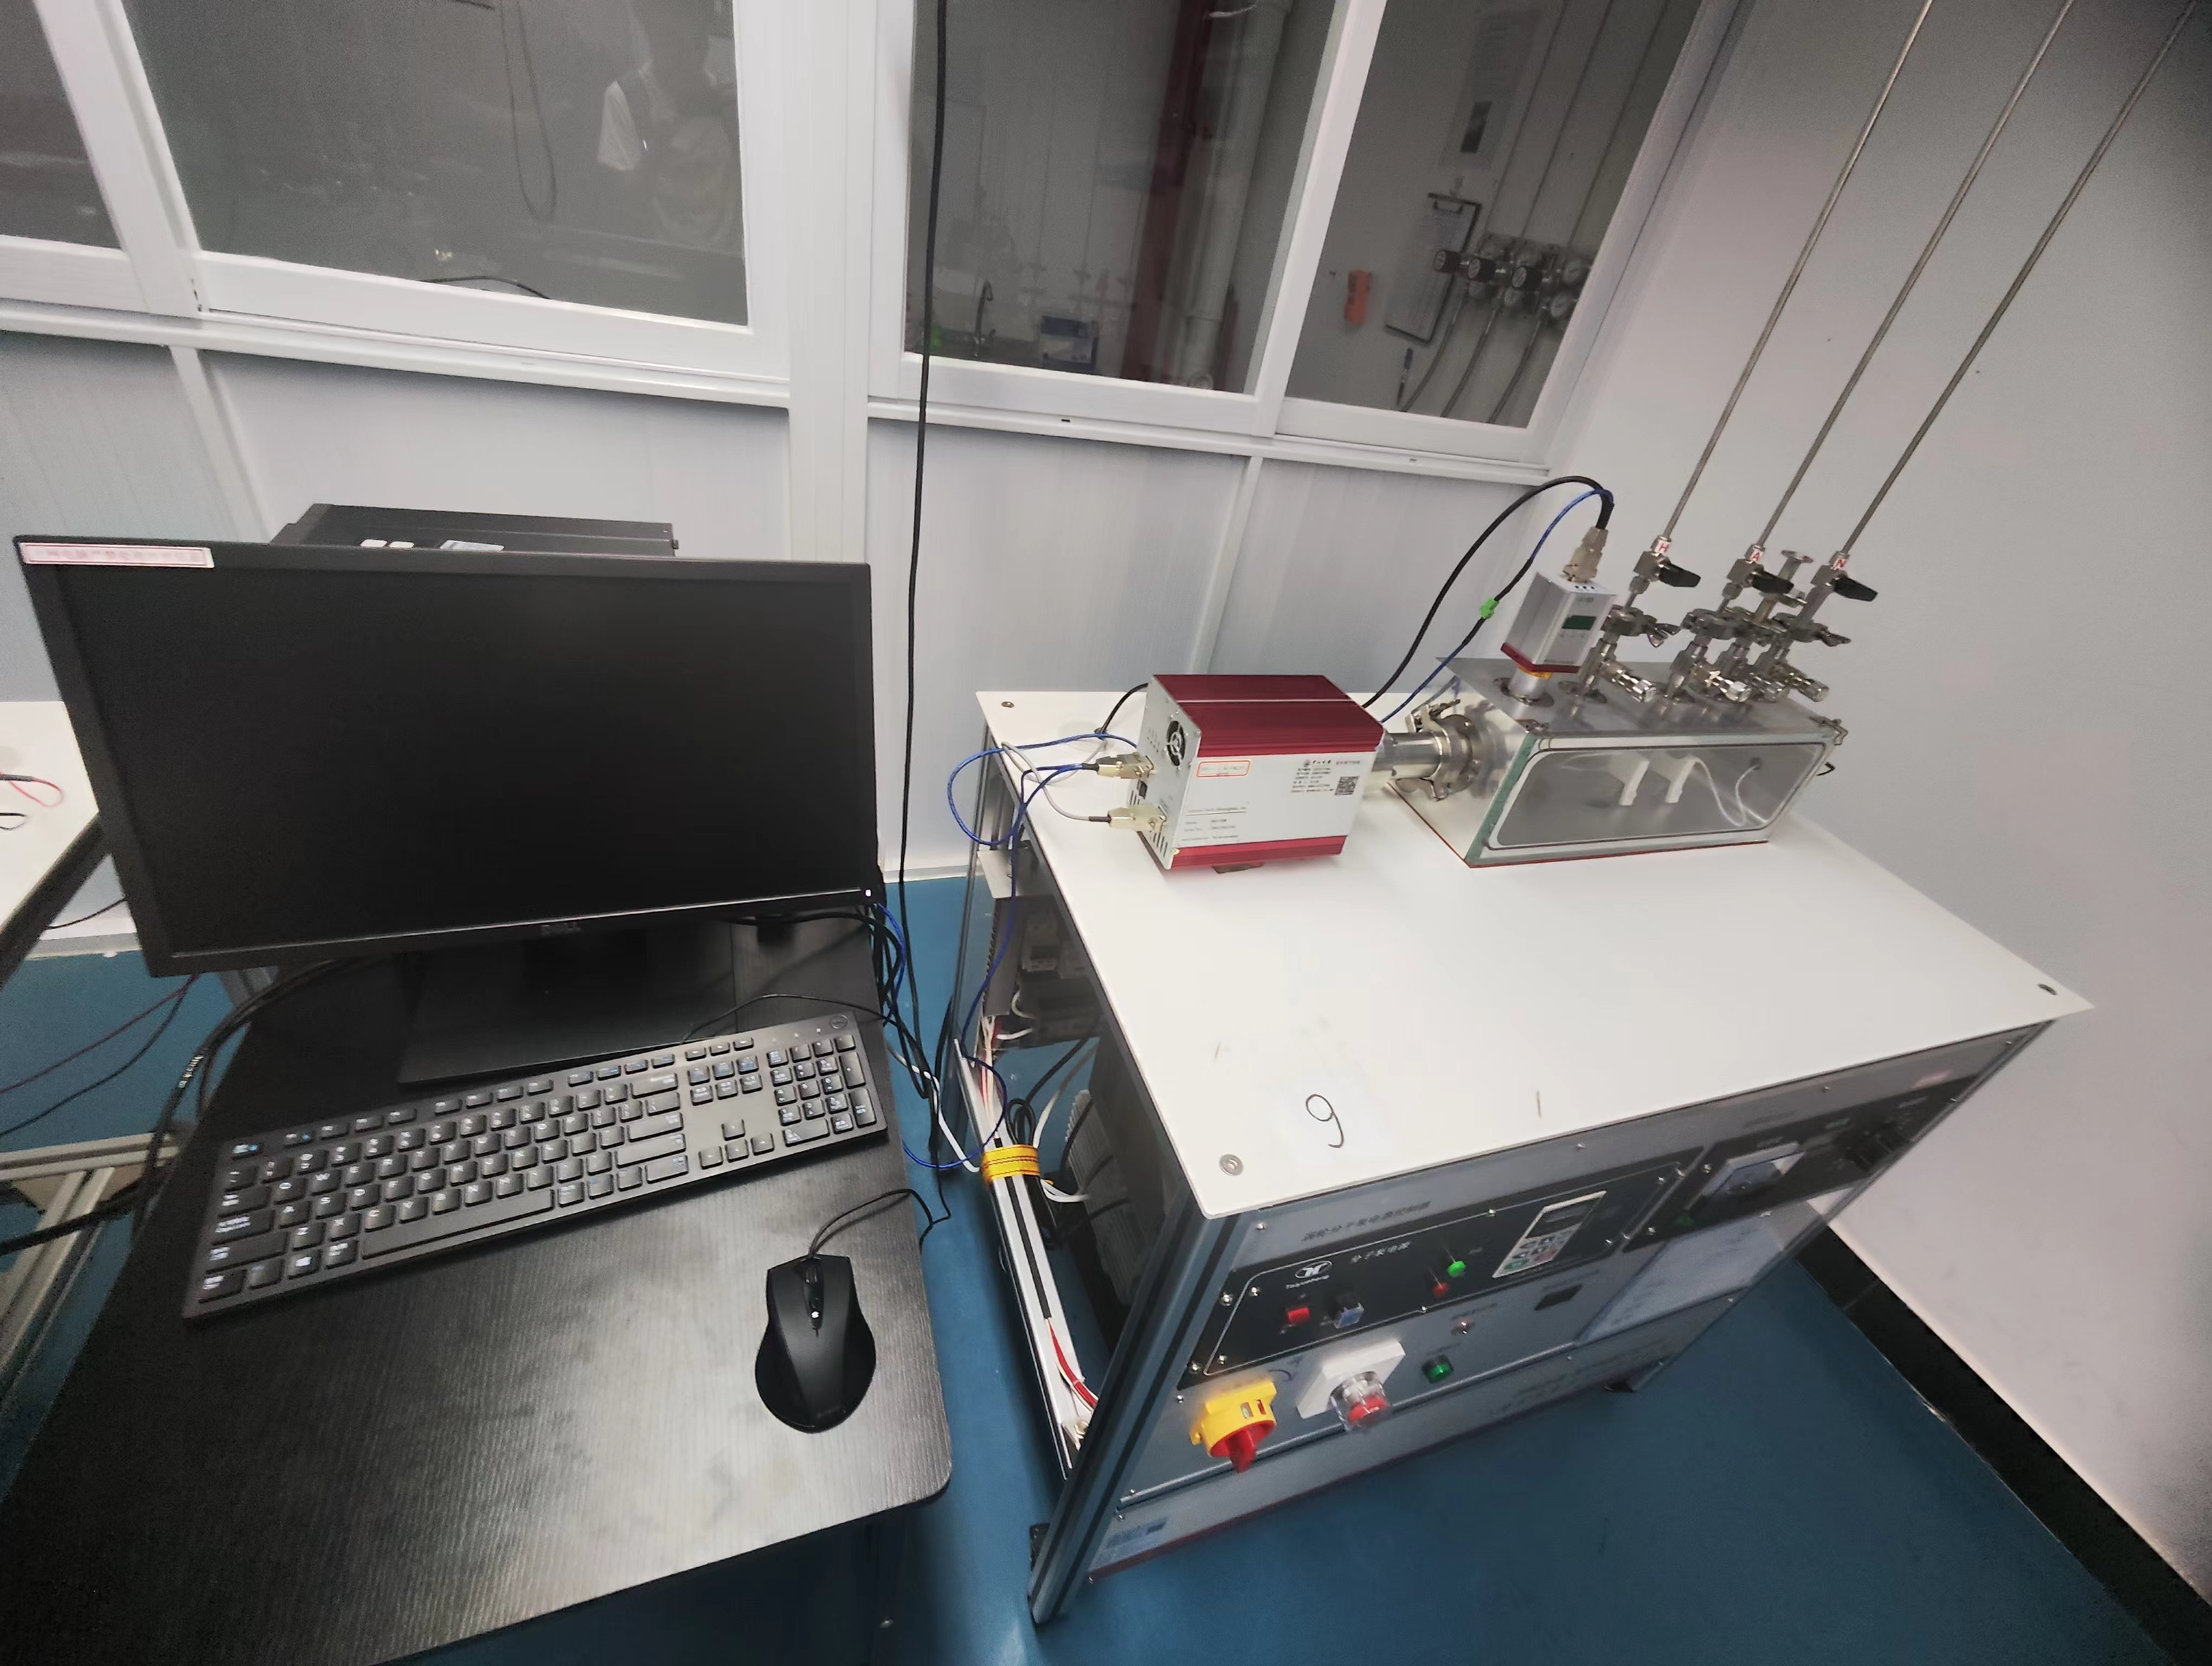
\includegraphics[width=0.5\linewidth]{桌面.jpg} % 这里的宽度可以根据需要调整
			\caption{桌面整理}
			\label{fig:desktop}
		\end{minipage}\hfill
		\begin{minipage}{0.45\textwidth}
			\centering
			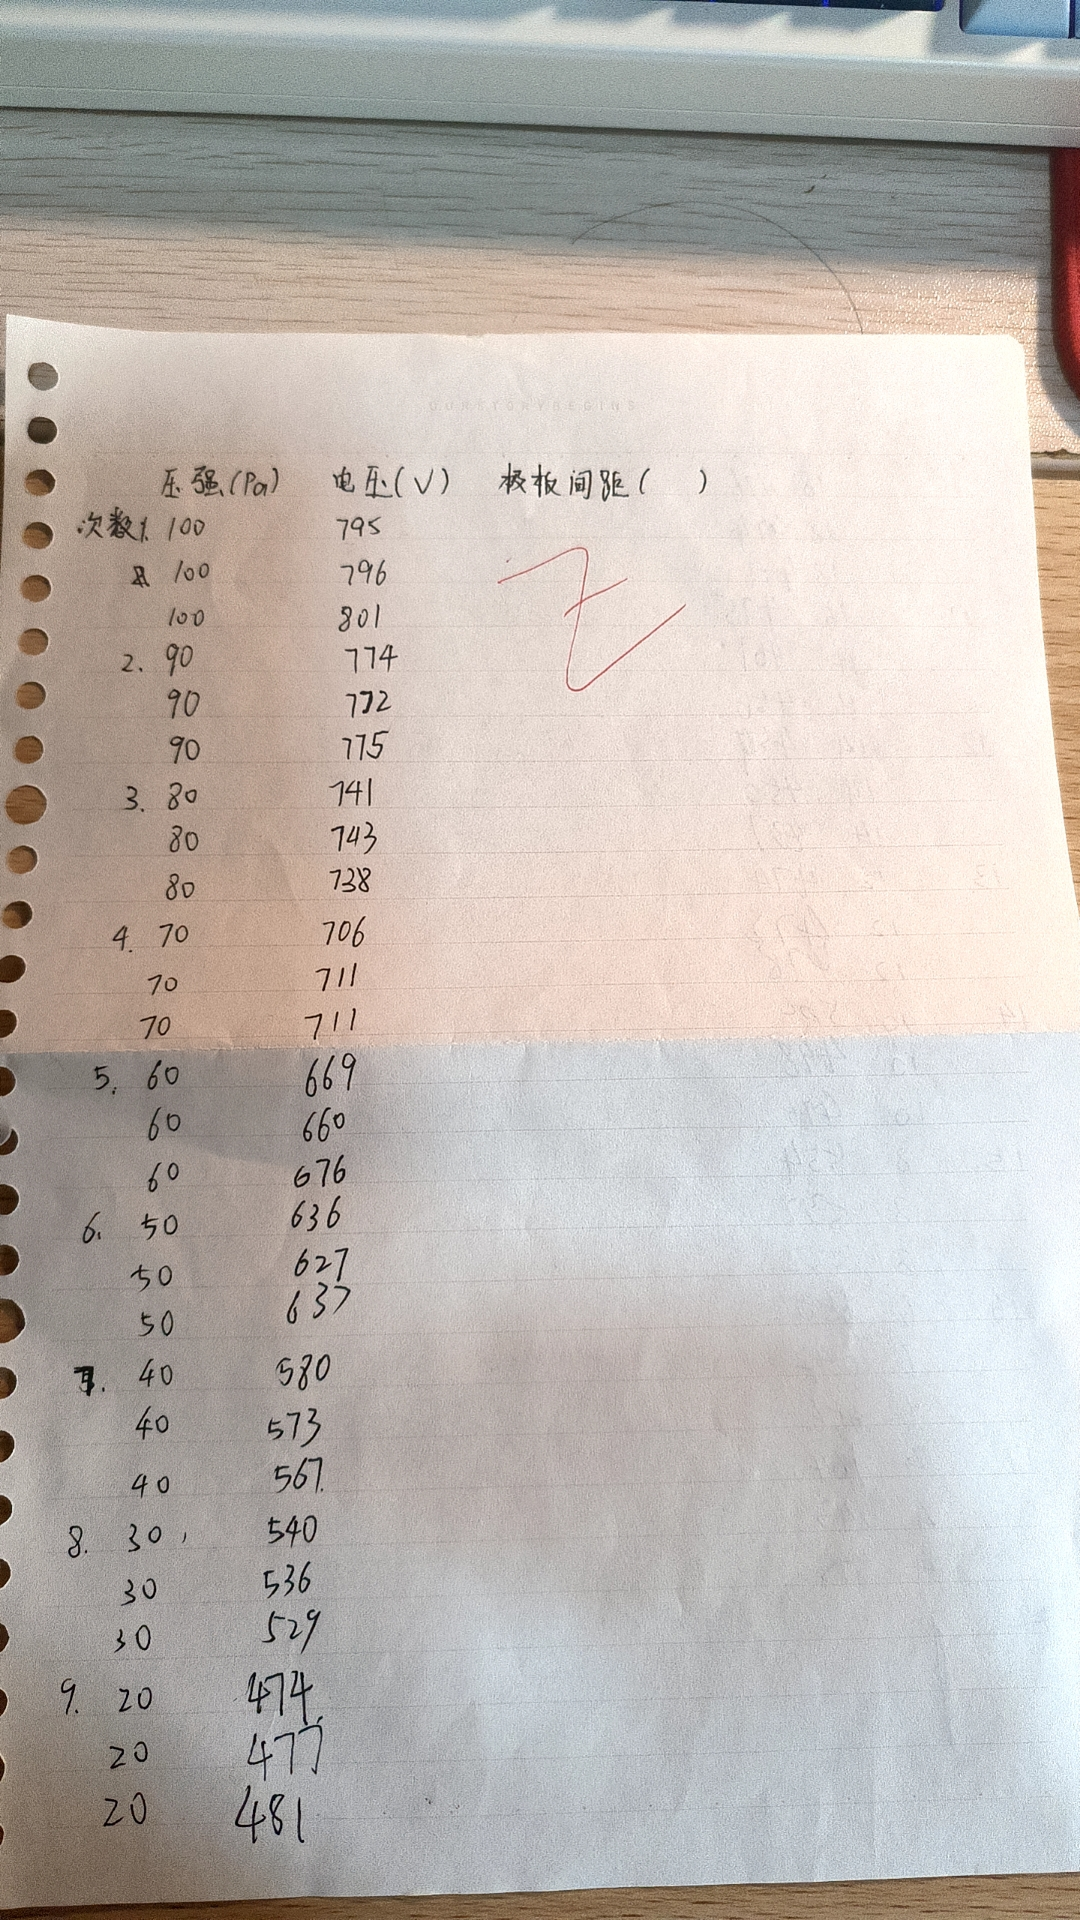
\includegraphics[width=0.5\linewidth]{签字111.jpg} % 这里的宽度可以根据需要调整
			\caption{实验数据签字}
			\label{fig:signature}
		\end{minipage}
	\end{figure}
	% ---
	
	
\end{document}